\section{Bereichssuchen}
\subsection{1D Bereichssuche}
\begin{frame}
	\frametitle{Bereichssuchen - Motivation}
	\begin{itemize}
		\item Datenbankabfrage
		\item Google Maps
	\end{itemize}
\end{frame}

\begin{frame}
	\frametitle{1D Bereichssuchen}
	Gegeben sind n verschiedene Zahlen $z_1, ... z_n$ und der Bereich [x,y].\\
	Gesucht sind nun die Zahlen $z_i$, die sich im Bereich [x,y] befinden \\
	\pause
	\textbf{Idee:} Sortiere die Zahlen und erstelle einen binären Baum. In diesem werden nun die Zahlen gesucht.
\end{frame}

\begin{frame}
	\frametitle{{1D Bereichssuchen}}
	\begin{figure}[htbp]
		\begin{center}
	  	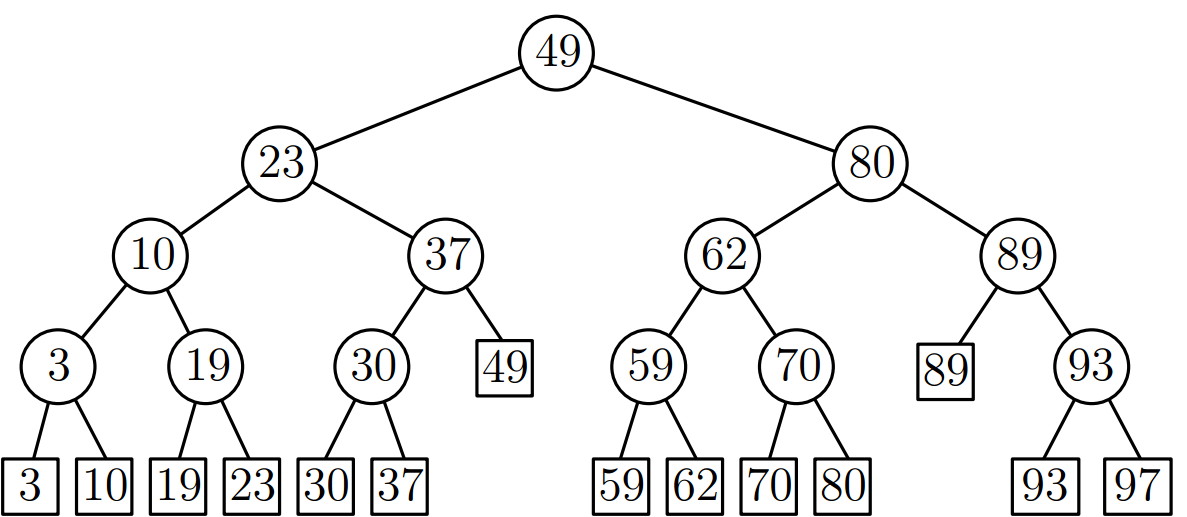
\includegraphics[width=.8\linewidth]{bilder/1d}
		\end{center}
	\end{figure}
	Binärer Baum zu den Zahlen 3, 10, 19, 23, 30, 37, 49, 59, 62, 70, 80, 89, 93, 97
\end{frame}

\begin{frame}
	\frametitle{{1D Bereichssuchen}}
\begin{figure}[htbp]
	\begin{center}
  	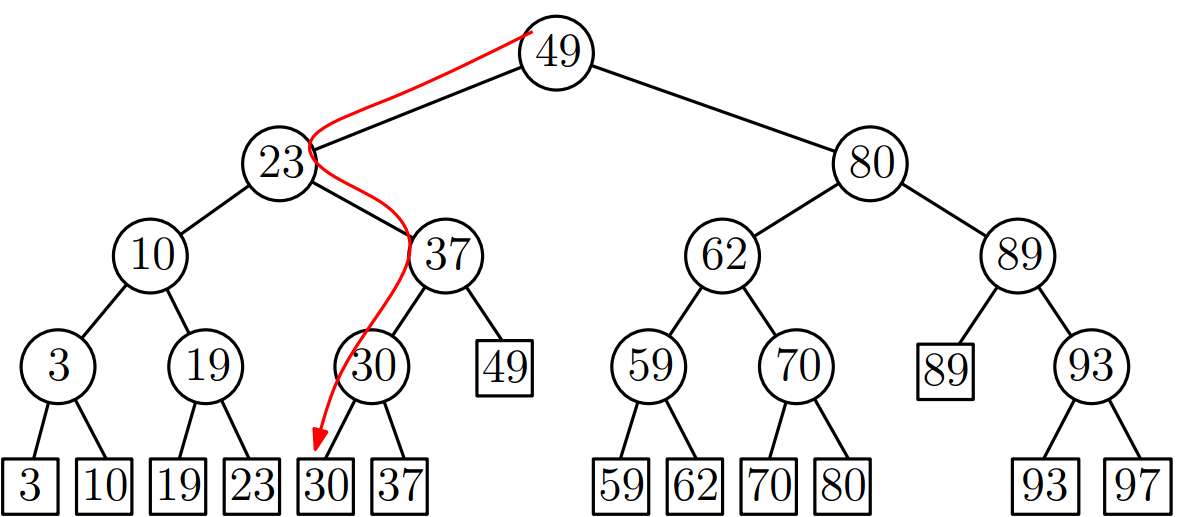
\includegraphics[width=.8\linewidth]{bilder/1d2}
	\end{center}
\end{figure}
Suchpfad für die Zahl 25
\end{frame}

\begin{frame}
	\frametitle{{1D Bereichssuchen}}
\begin{figure}[htbp]
	\begin{center}
  	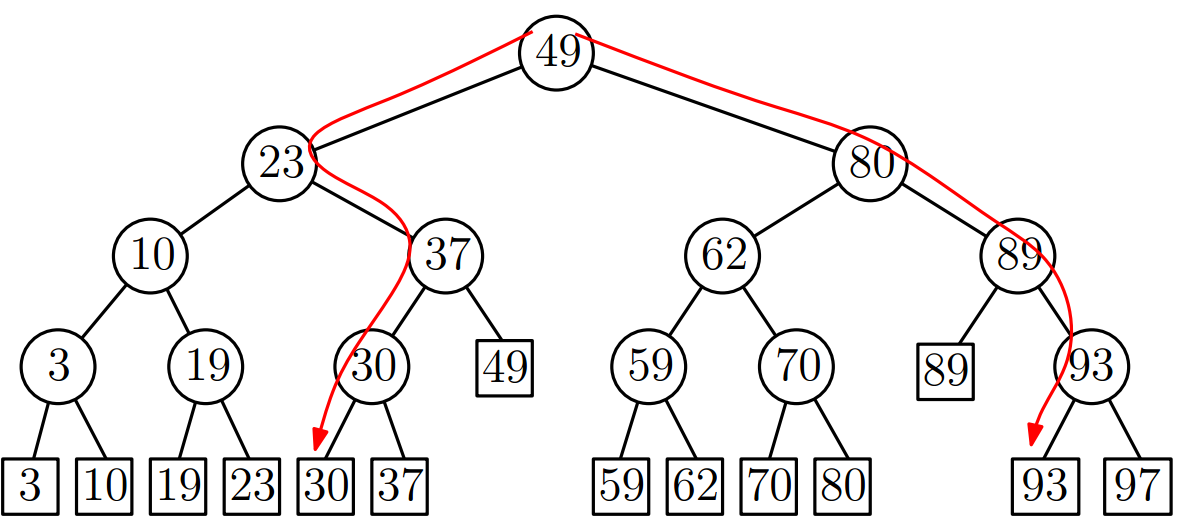
\includegraphics[width=.8\linewidth]{bilder/1d3}
	\end{center}
\end{figure}
Suchpfad für 25 und 90
\end{frame}

\begin{frame}
	\frametitle{{1D Bereichssuchen}}
\begin{figure}[htbp]
	\begin{center}
  	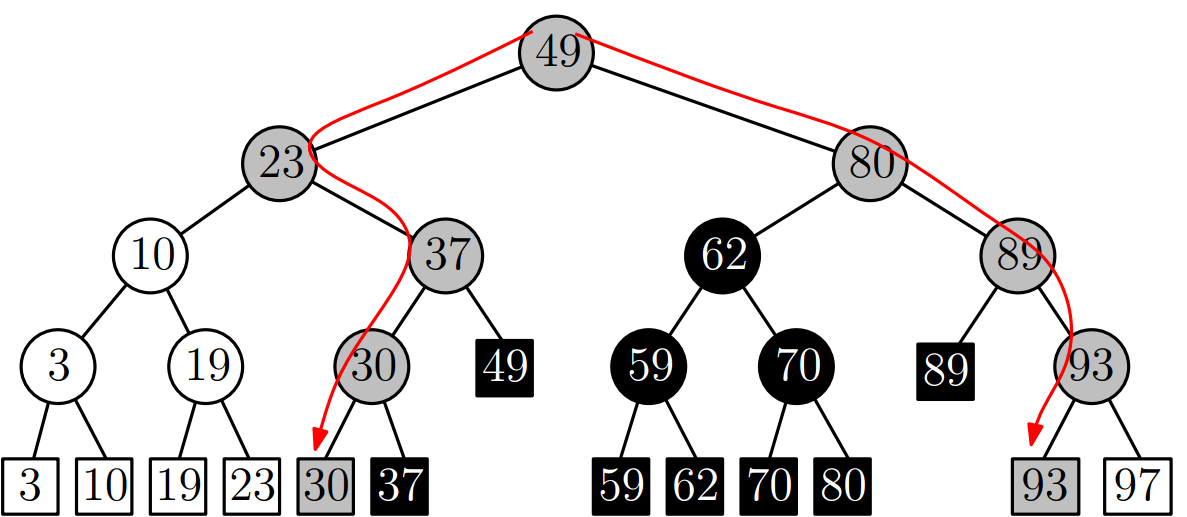
\includegraphics[width=.8\linewidth]{bilder/1d4}
	\end{center}
\end{figure}
Bereichssuche für [25, 90]
\end{frame}

\begin{frame}
	\frametitle{{1D Bereichssuchen}}
	\textbf{Weiße Knoten: } werden für die Suche nie betrachtet\\
	\textbf{Graue Knoten: } wurden besucht, es ist aber unklar, ob sie zur Ausgabe gehören\\
	\textbf{Schwarze Knoten: } wurden besucht und gesamter Unterteilbaum gehört zur Ausgabe.
\end{frame}

\begin{frame}
	\frametitle{{1D Bereichssuchen}}
\begin{figure}[htbp]
	\begin{center}
  	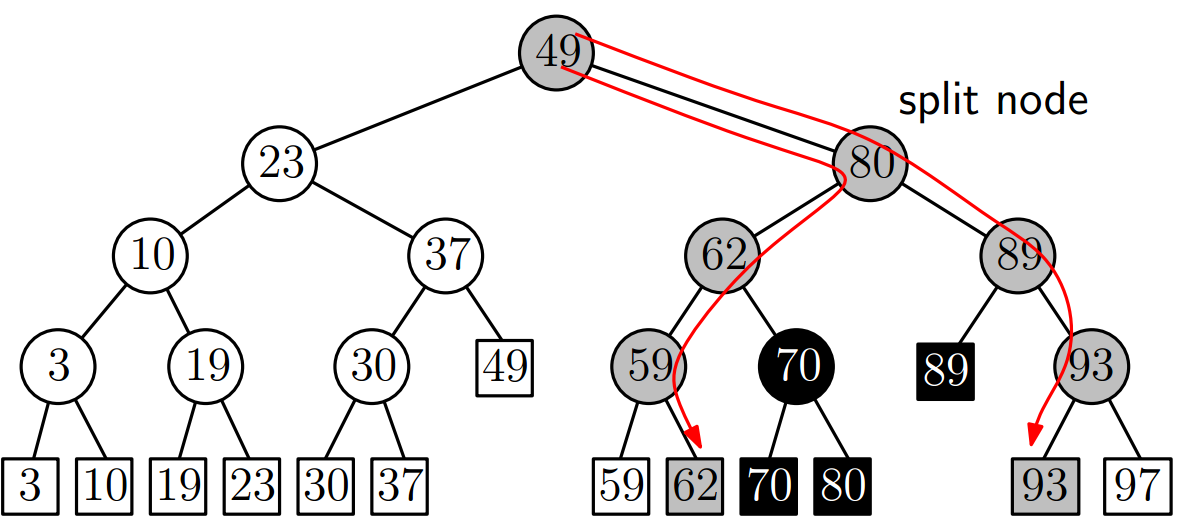
\includegraphics[width=.8\linewidth]{bilder/1d5}
	\end{center}
\end{figure}
Bereichssuche für [61, 90]
\end{frame}


\begin{frame}
	\frametitle{1D Bereichssuchen - SplitNode}
	Sei $T$ der Baum und $x, x'$ zwei Werte mit $x \leq x'$\newline\newline
	$FindeSplitNode(T, x, x')$\\
	\begin{algorithmic}
	\State $v \gets root(T)$
	\pause
	\While{v ist kein Blatt und ($x' \leq x_v \mbox{ oder } x>x_v$)}
		\If{$x' \leq x_v$}
			\State $v \gets lc(v)$
			\pause
		\Else
			\State $v \gets rc(v)$
		\EndIf
	\EndWhile
	\State \Return $v$
	\end{algorithmic}
\end{frame}

\begin{frame}
	\frametitle{1D Bereichssuchen - Pseudocode}
	$1DBereichssuche(T,x,x')$
	\begin{algorithmic}
	\State $v_{split} \gets FindSplitNode(T, x, x')$
	\If {$v_{split} \mbox{ist ein Blatt}$}
		\State $\mbox{Prüfe ob }v_{split} \mbox{ gemeldet werden muss}$
		\pause
	\Else
		\State $v \gets lc(v_{split})$
		\While {$\mbox{v ist kein Blatt}$}
			\If{$x \leq x_v$}
				\State $meldeTeilbaum(rc(v))$
				\State $v \gets lc(v)$
				\pause
			\Else 
				\State $v\gets rc(v)$
			\EndIf
		\EndWhile
		\pause
		\State $\mbox{Prüfe, ob v gemeldet werden muss}$
		\pause
		\State $\mbox{mache das gleiche noch äquivalent mit x'...}$
	\EndIf
	\end{algorithmic}

\end{frame}

\begin{frame}
	\frametitle{1D Bereichssuchen - Laufzeit}
	\textbf{Graue Knoten: } Es gibt genau zwei Pfade mit grauen Knoten. Da der Baum balanciert ist $\Rightarrow O(log(n))$\\
	\pause
	\textbf{Schwarze Knoten: } Ein Teilbaum mit k Knoten hat k-1 interne Knoten. Wir finden also k Knoten durch das Traversieren $\Rightarrow O(k)$\newline
	\newline
	 \pause
	$\Rightarrow O(log(n) + k)$ \newline
	\newline
	\pause
	Der Baum muss allerdings auch erstmal erstellt werden. Das liegt in $O(n)$.
\end{frame}
\subsection{kd-Baum}
\begin{frame}
	\frametitle{kd-Baum}
	Im 2-dimensionalen sind Bereichssuchen ähnlich zu machen. \\
	Dafür werden \textbf{kd-Bäume} benutzt.
	\begin{figure}[htbp]
	\begin{center}
  	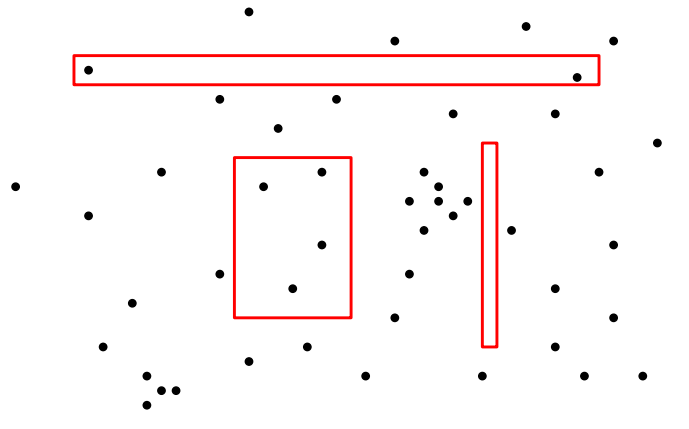
\includegraphics[width=.8\linewidth]{bilder/2d.png}
	\end{center}
\end{figure}
\end{frame}

\begin{frame}
	\frametitle{kd-Baum - Die Idee}
	Wir bauen einen Baum ähnlich wie den für die 1-D Suche. Da wir im 2D x und y betrachten müssen, splitten wir beim kd-Baum nacheinander erst nach x und dann nach y auf.
\end{frame}

\begin{frame}
	\frametitle{kd-Baum}
	\only<1>{
		\begin{figure}
		\mbox{
			\subfigure{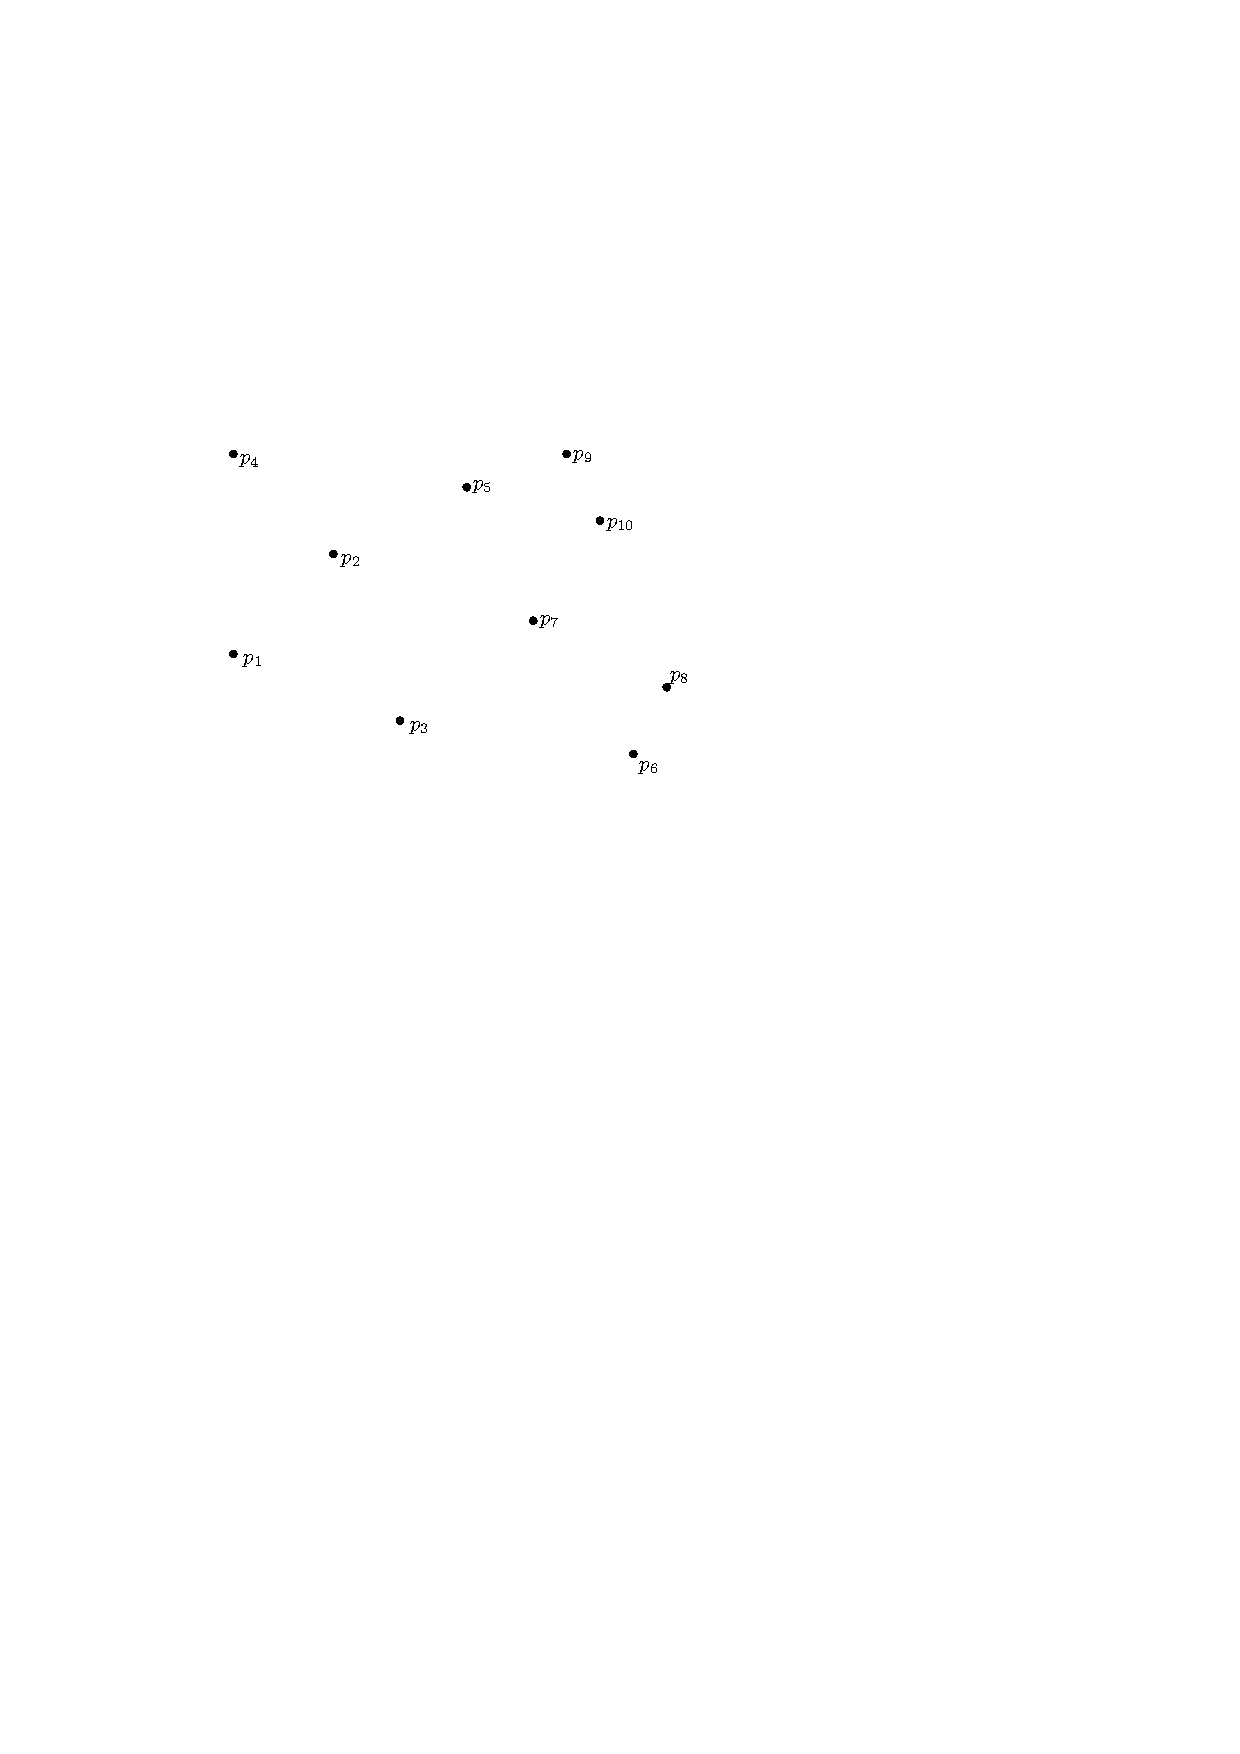
\includegraphics[width=.45\linewidth]{bilder/kd0}}\quad
			\subfigure{
\includegraphics[width=.5\linewidth]{bilder/kdtree0}}
			}
	\end{figure}
	}
	\only<2>{
		\begin{figure}
		\mbox{
			\subfigure{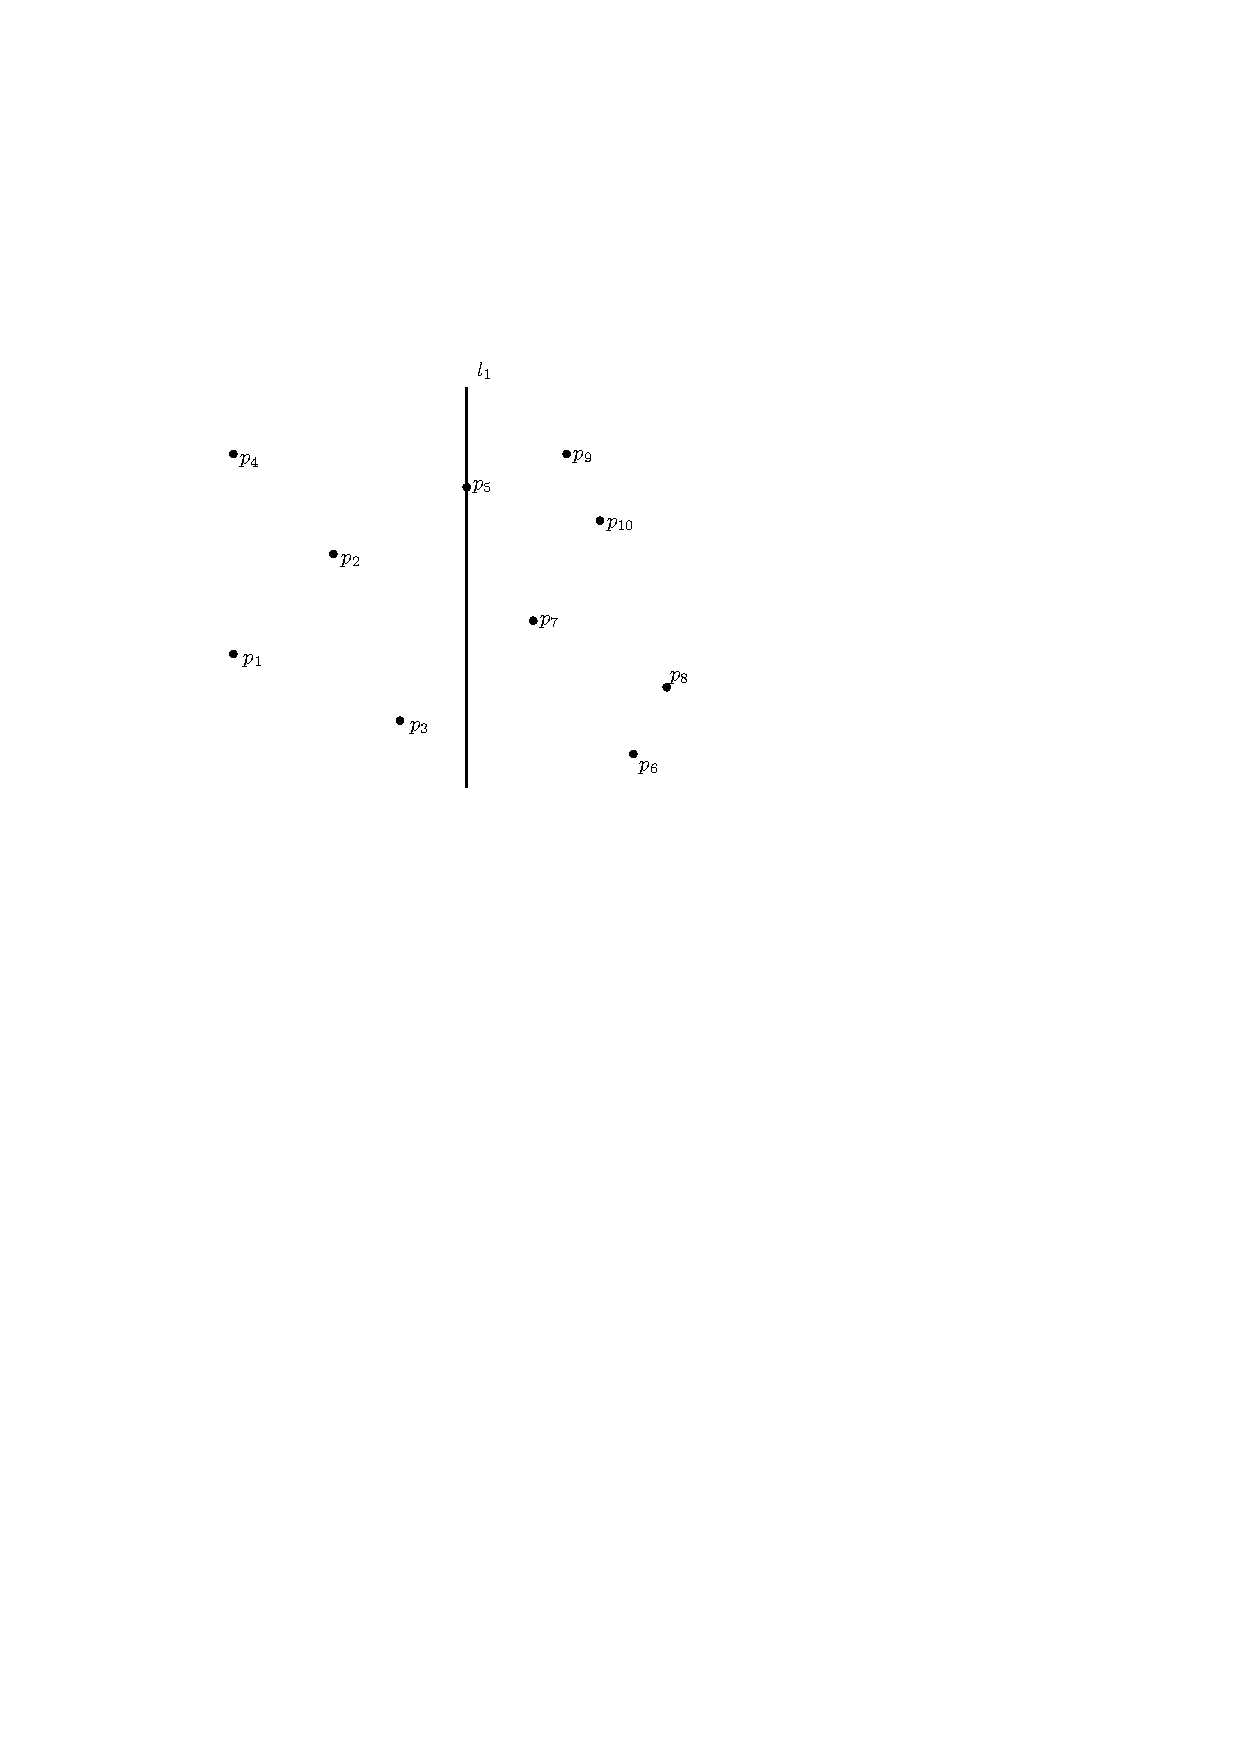
\includegraphics[width=.45\linewidth]{bilder/kd1}}\quad
			\subfigure{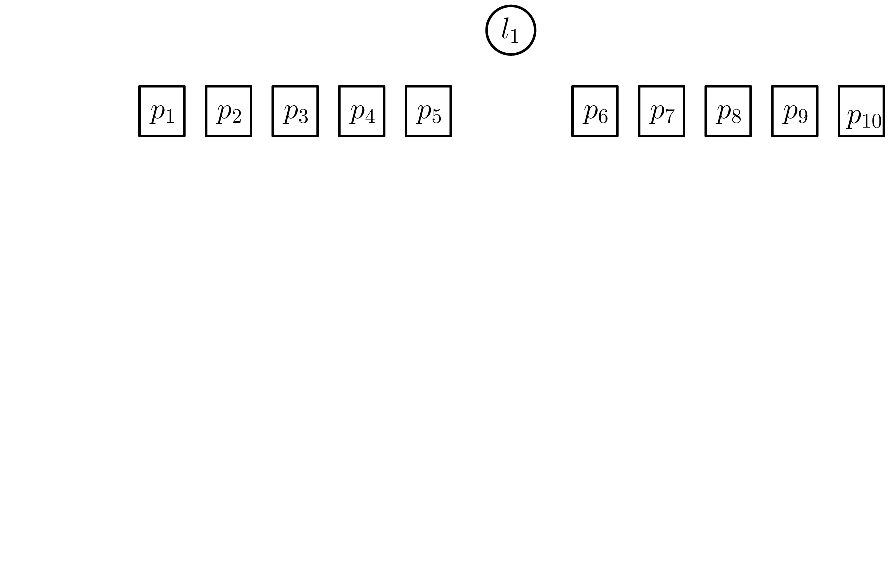
\includegraphics[width=.5\linewidth]{bilder/kdtree1}}
			}
	\end{figure}
	}
	\only<3>{
		\begin{figure}
		\mbox{
			\subfigure{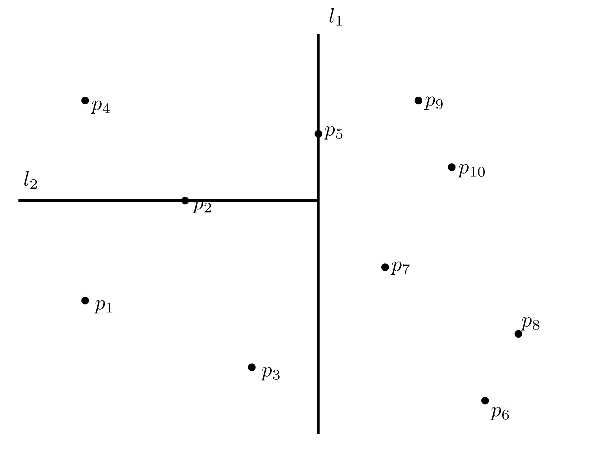
\includegraphics[width=.45\linewidth]{bilder/kd2}}\quad
			\subfigure{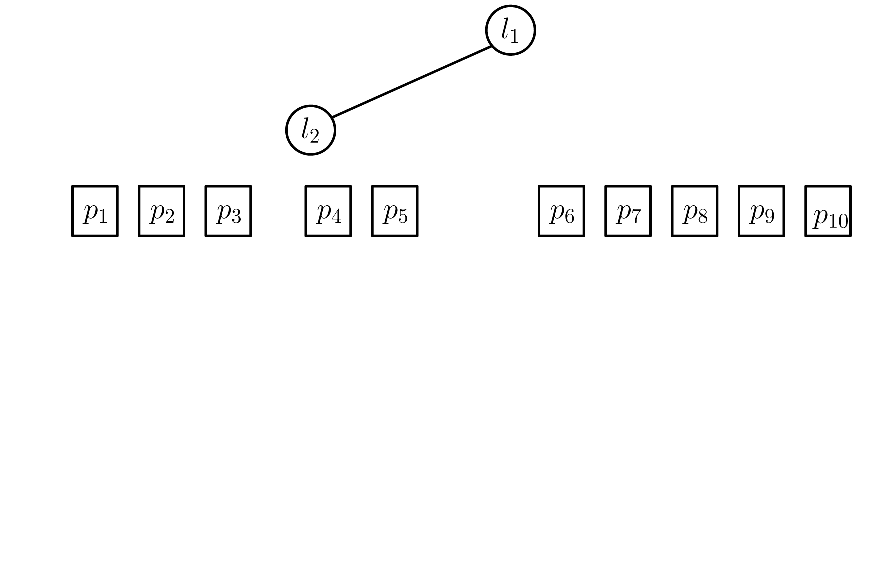
\includegraphics[width=.5\linewidth]{bilder/kdtree2}}
			}
	\end{figure}
	}
	\only<4>{
		\begin{figure}
		\mbox{
			\subfigure{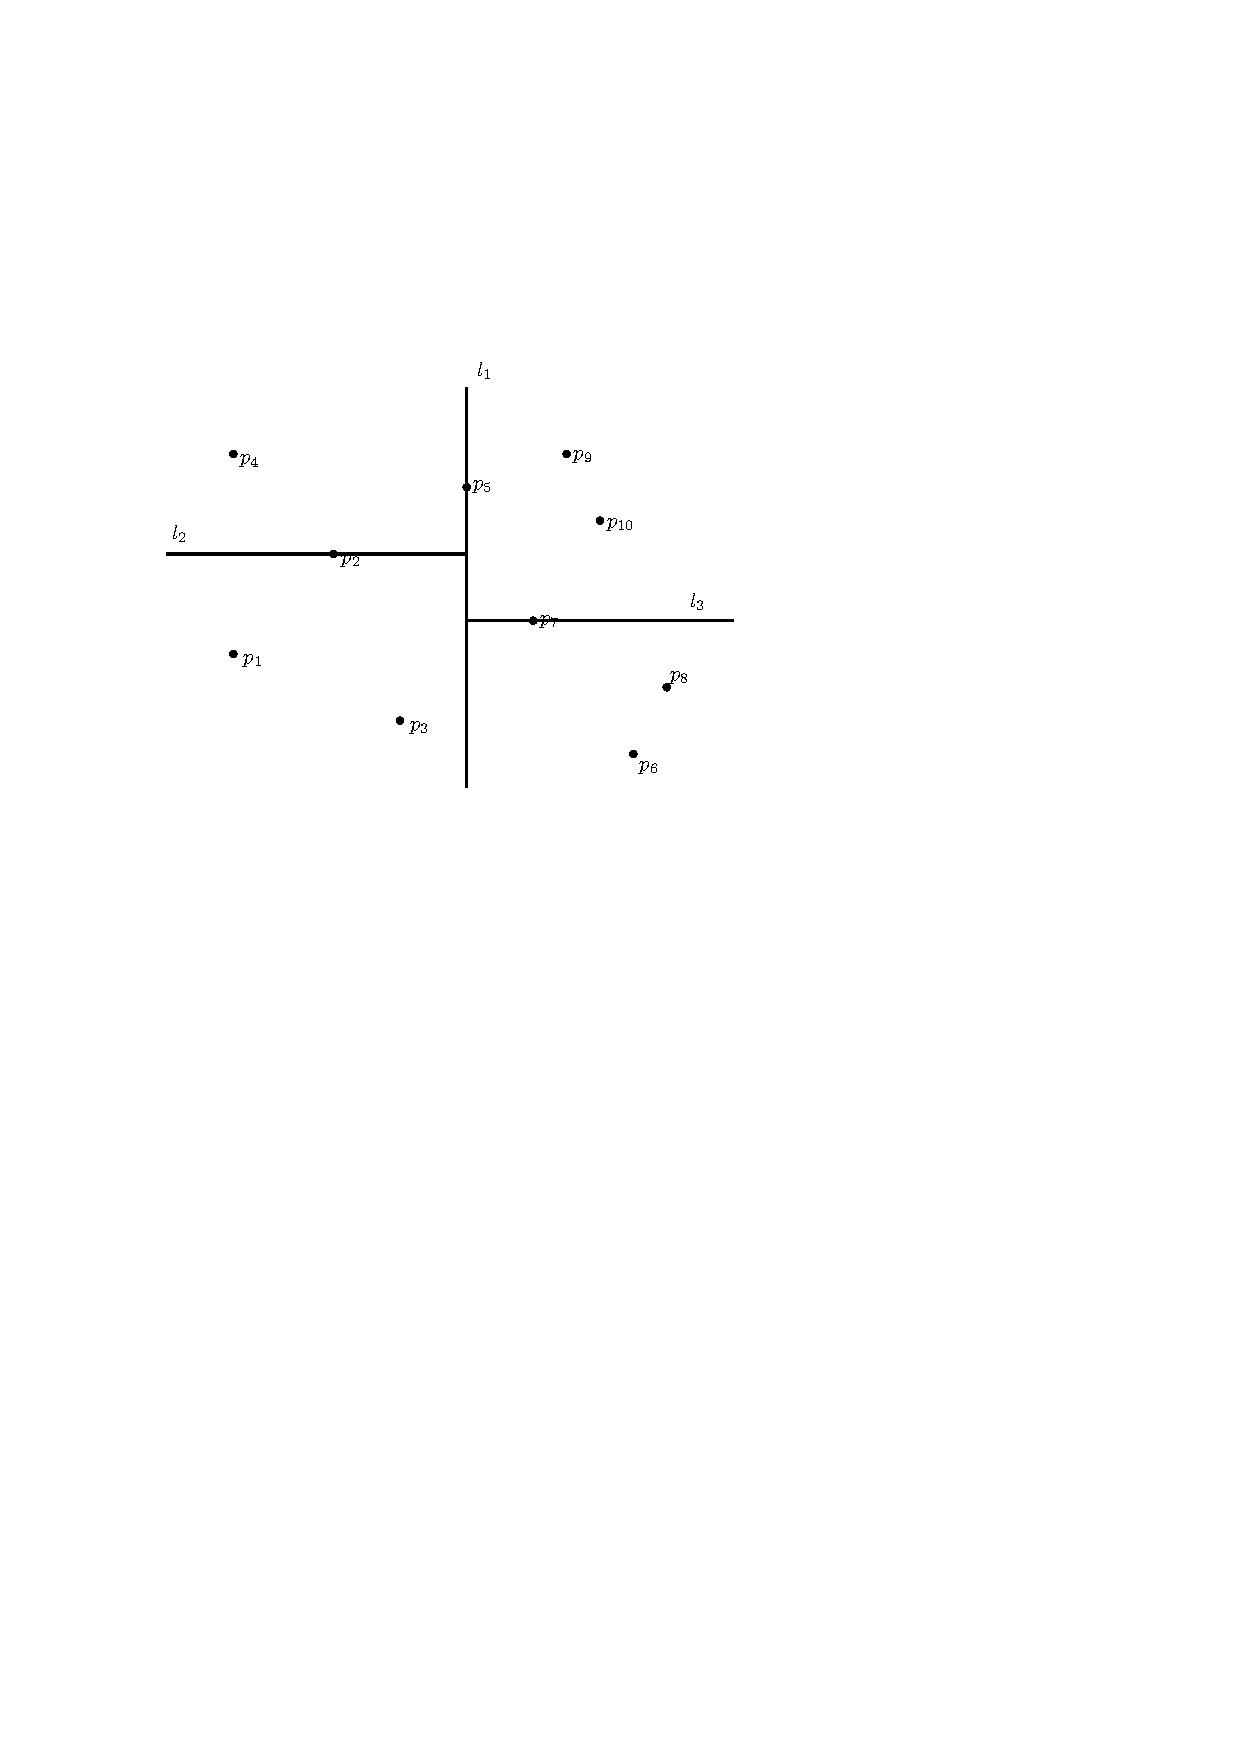
\includegraphics[width=.45\linewidth]{bilder/kd3}}\quad
			\subfigure{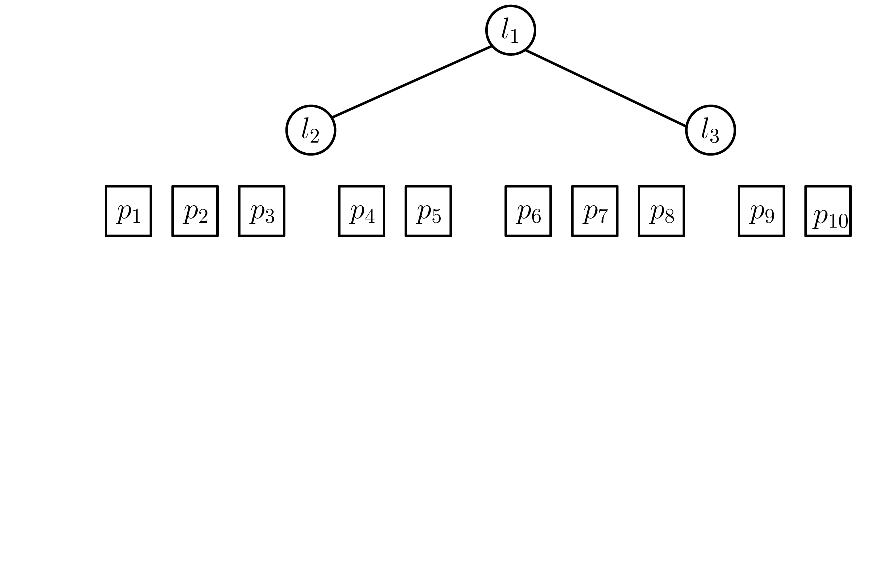
\includegraphics[width=.5\linewidth]{bilder/kdtree3}}
			}
	\end{figure}
	}
	\only<5>{
		\begin{figure}
		\mbox{
			\subfigure{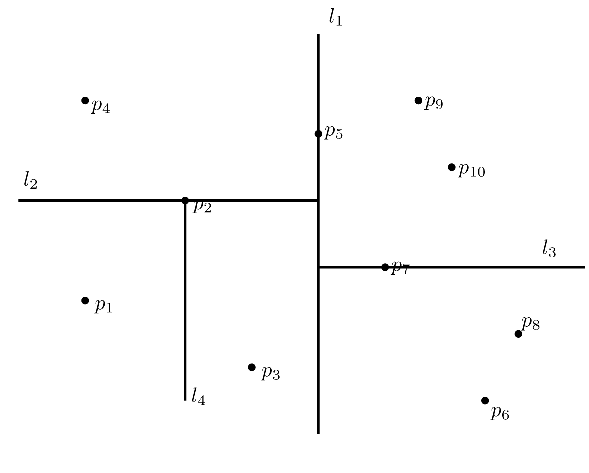
\includegraphics[width=.45\linewidth]{bilder/kd4}}\quad
			\subfigure{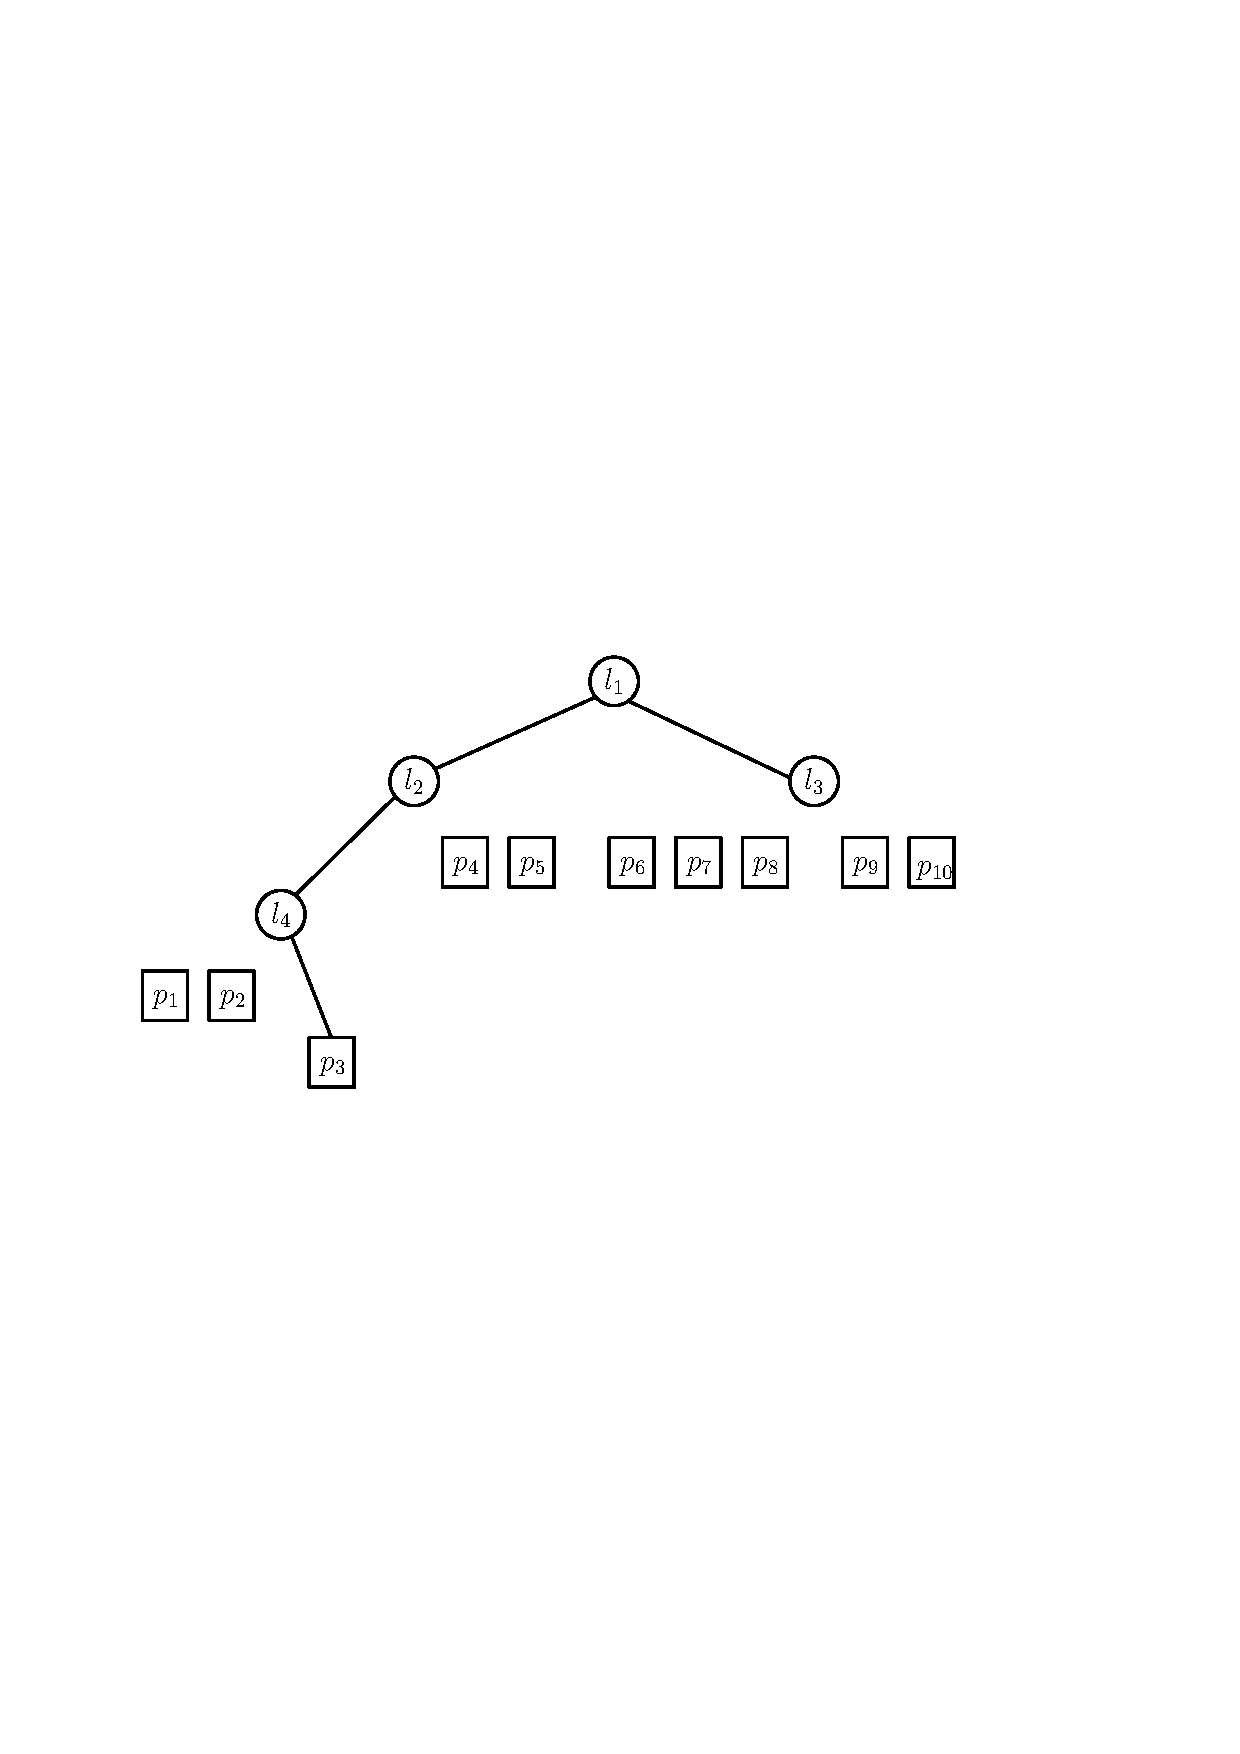
\includegraphics[width=.5\linewidth]{bilder/kdtree4}}
			}
	\end{figure}
	}
	\only<6>{
		\begin{figure}
		\mbox{
			\subfigure{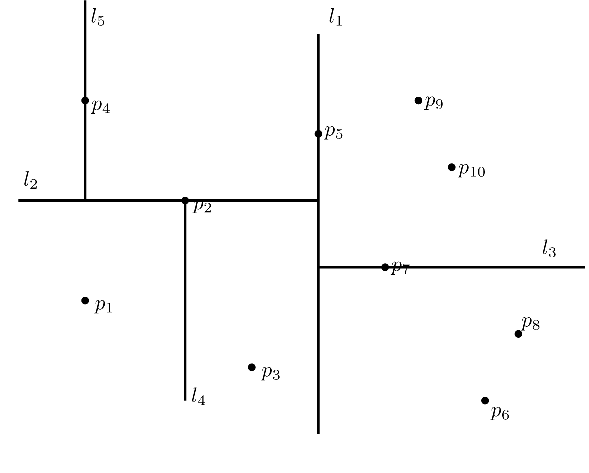
\includegraphics[width=.45\linewidth]{bilder/kd5}}\quad
			\subfigure{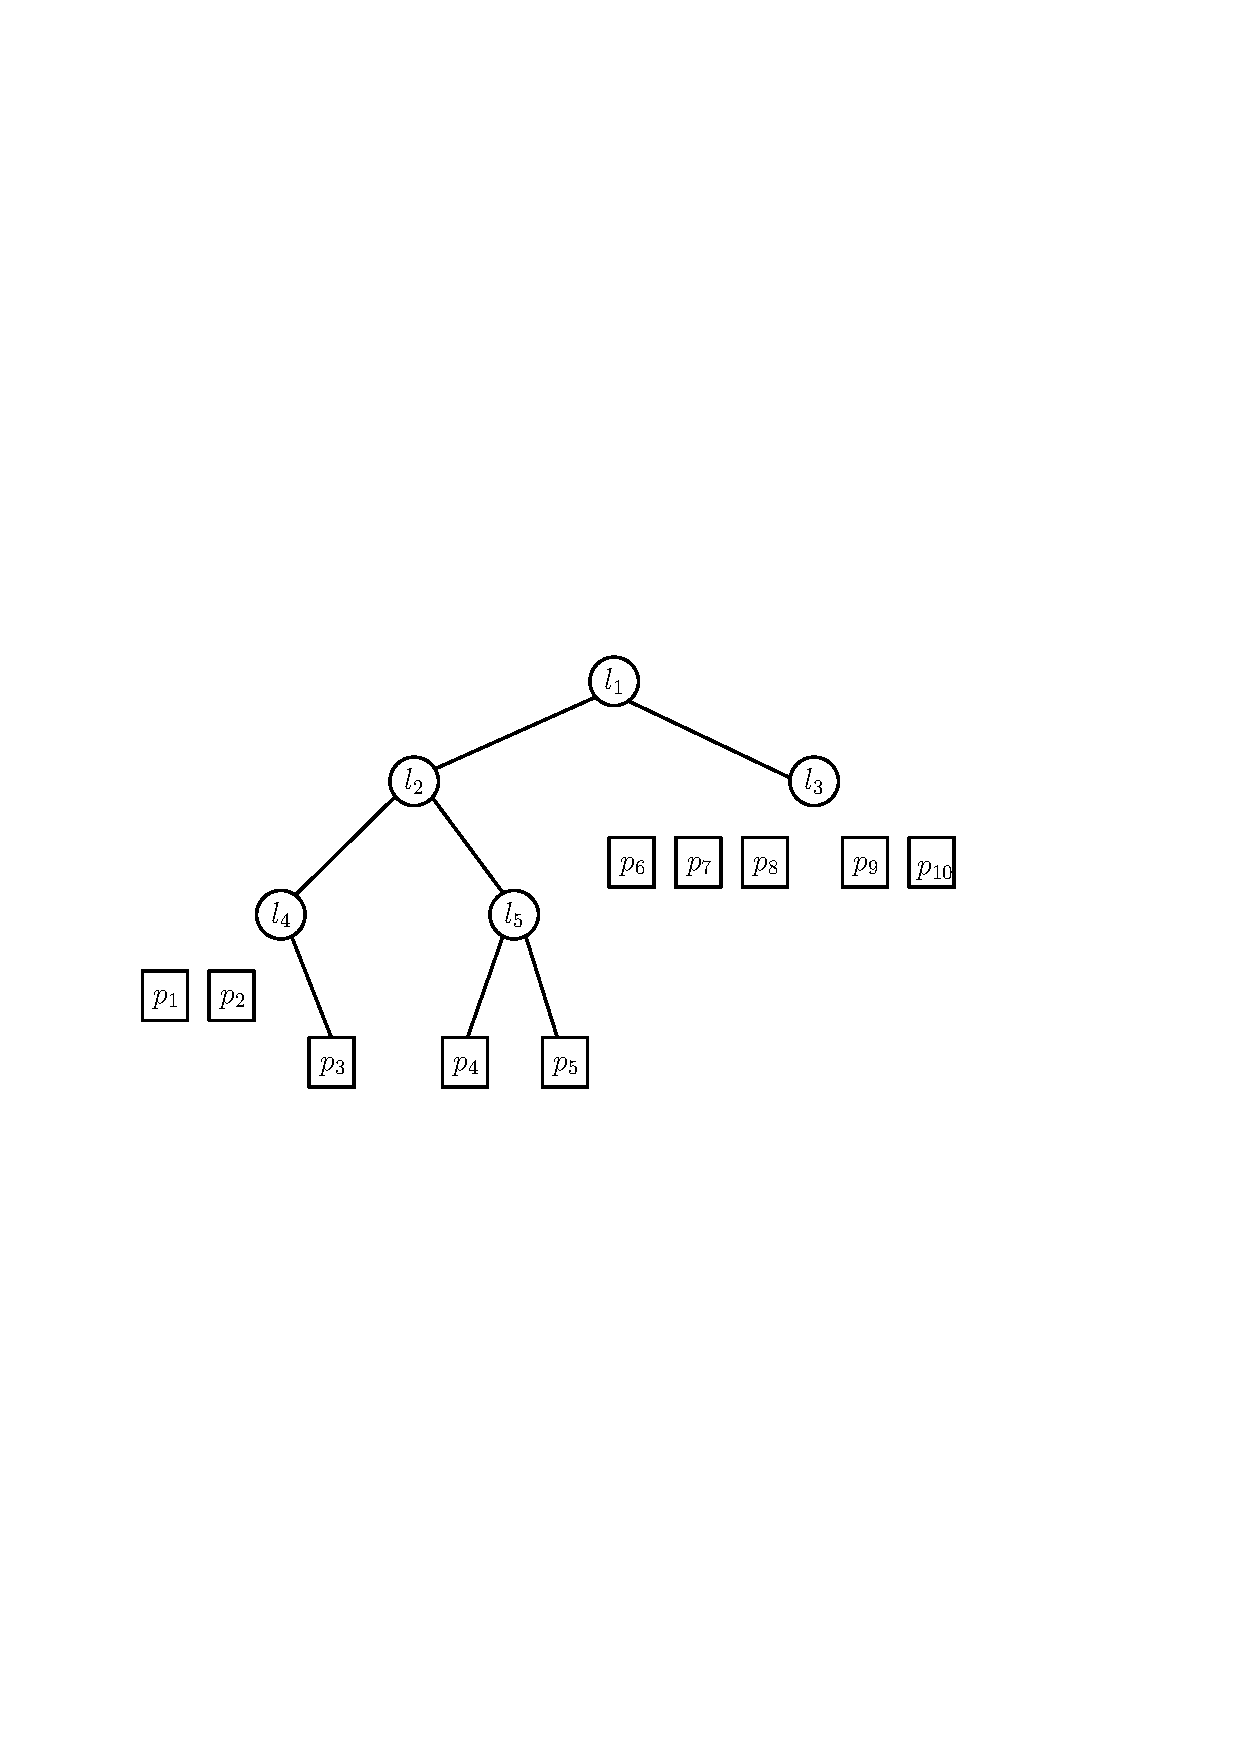
\includegraphics[width=.5\linewidth]{bilder/kdtree5}}
			}
	\end{figure}
	}
	\only<7>{
		\begin{figure}
		\mbox{
			\subfigure{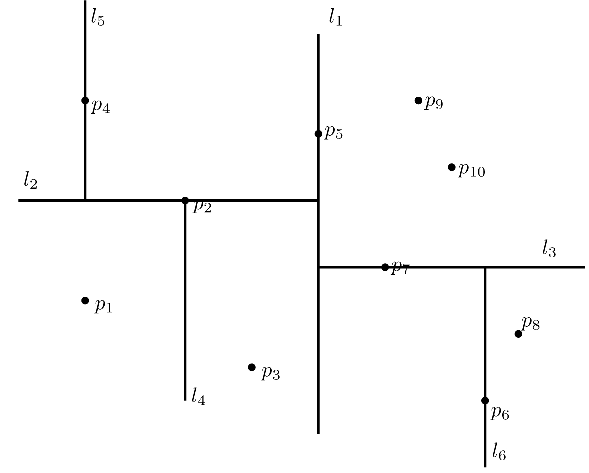
\includegraphics[width=.45\linewidth]{bilder/kd6}}\quad
			\subfigure{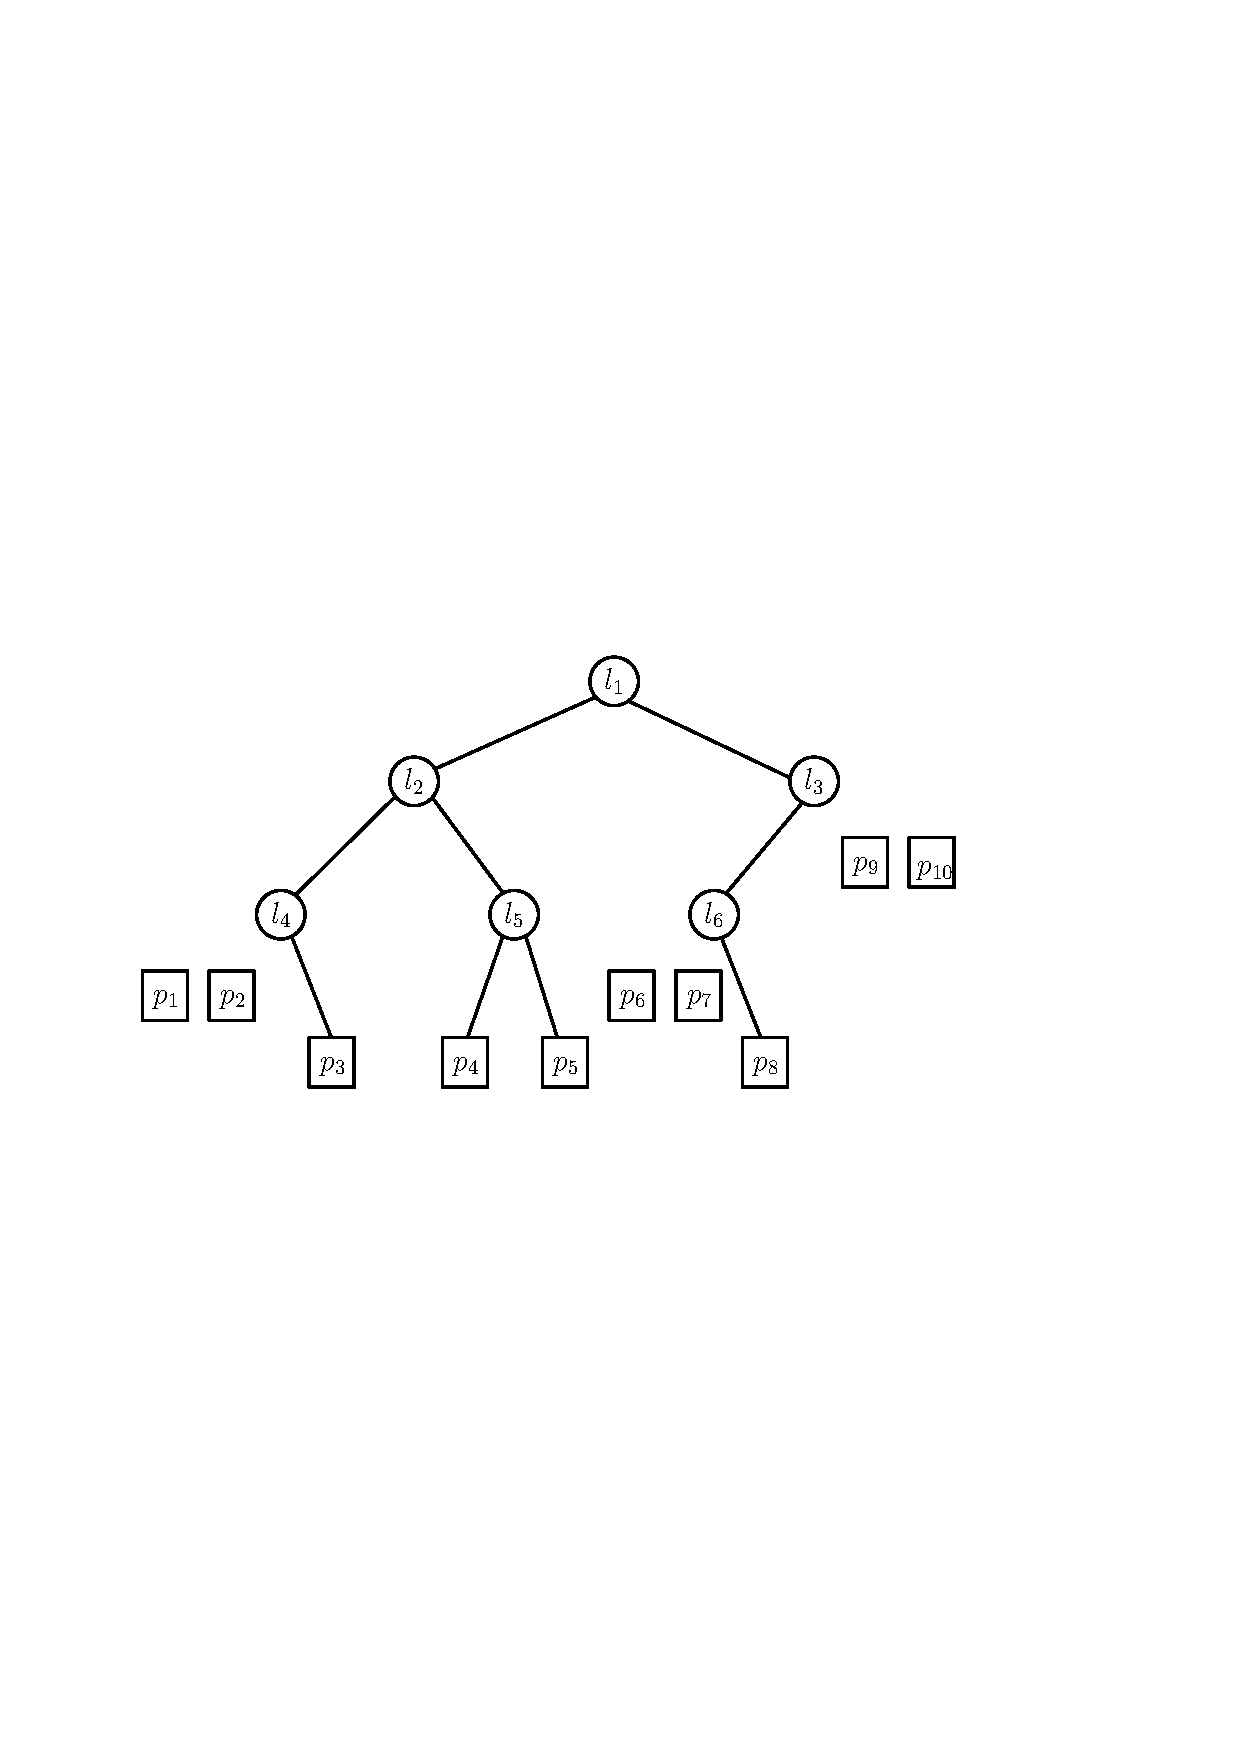
\includegraphics[width=.5\linewidth]{bilder/kdtree6}}
			}
	\end{figure}
	}
	\only<8>{
		\begin{figure}
		\mbox{
			\subfigure{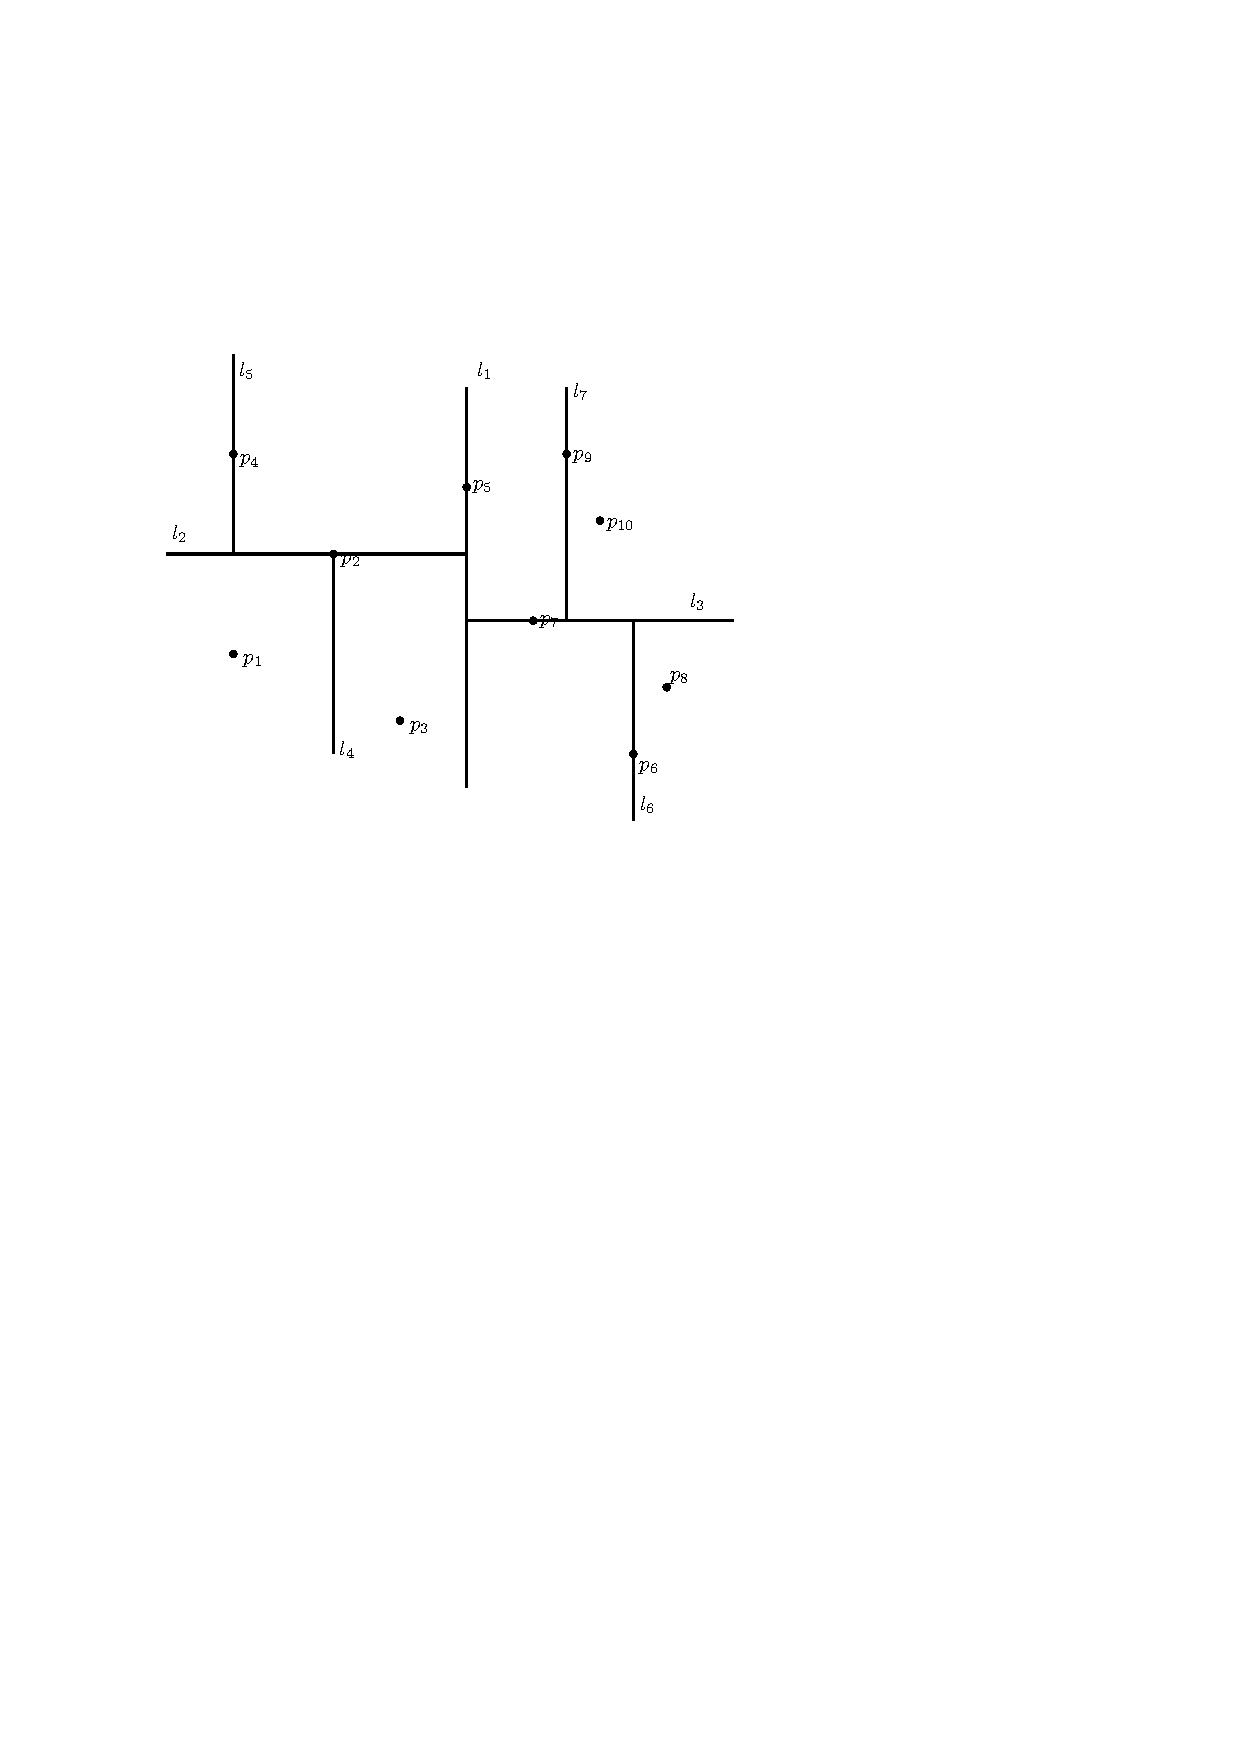
\includegraphics[width=.45\linewidth]{bilder/kd7}}\quad
			\subfigure{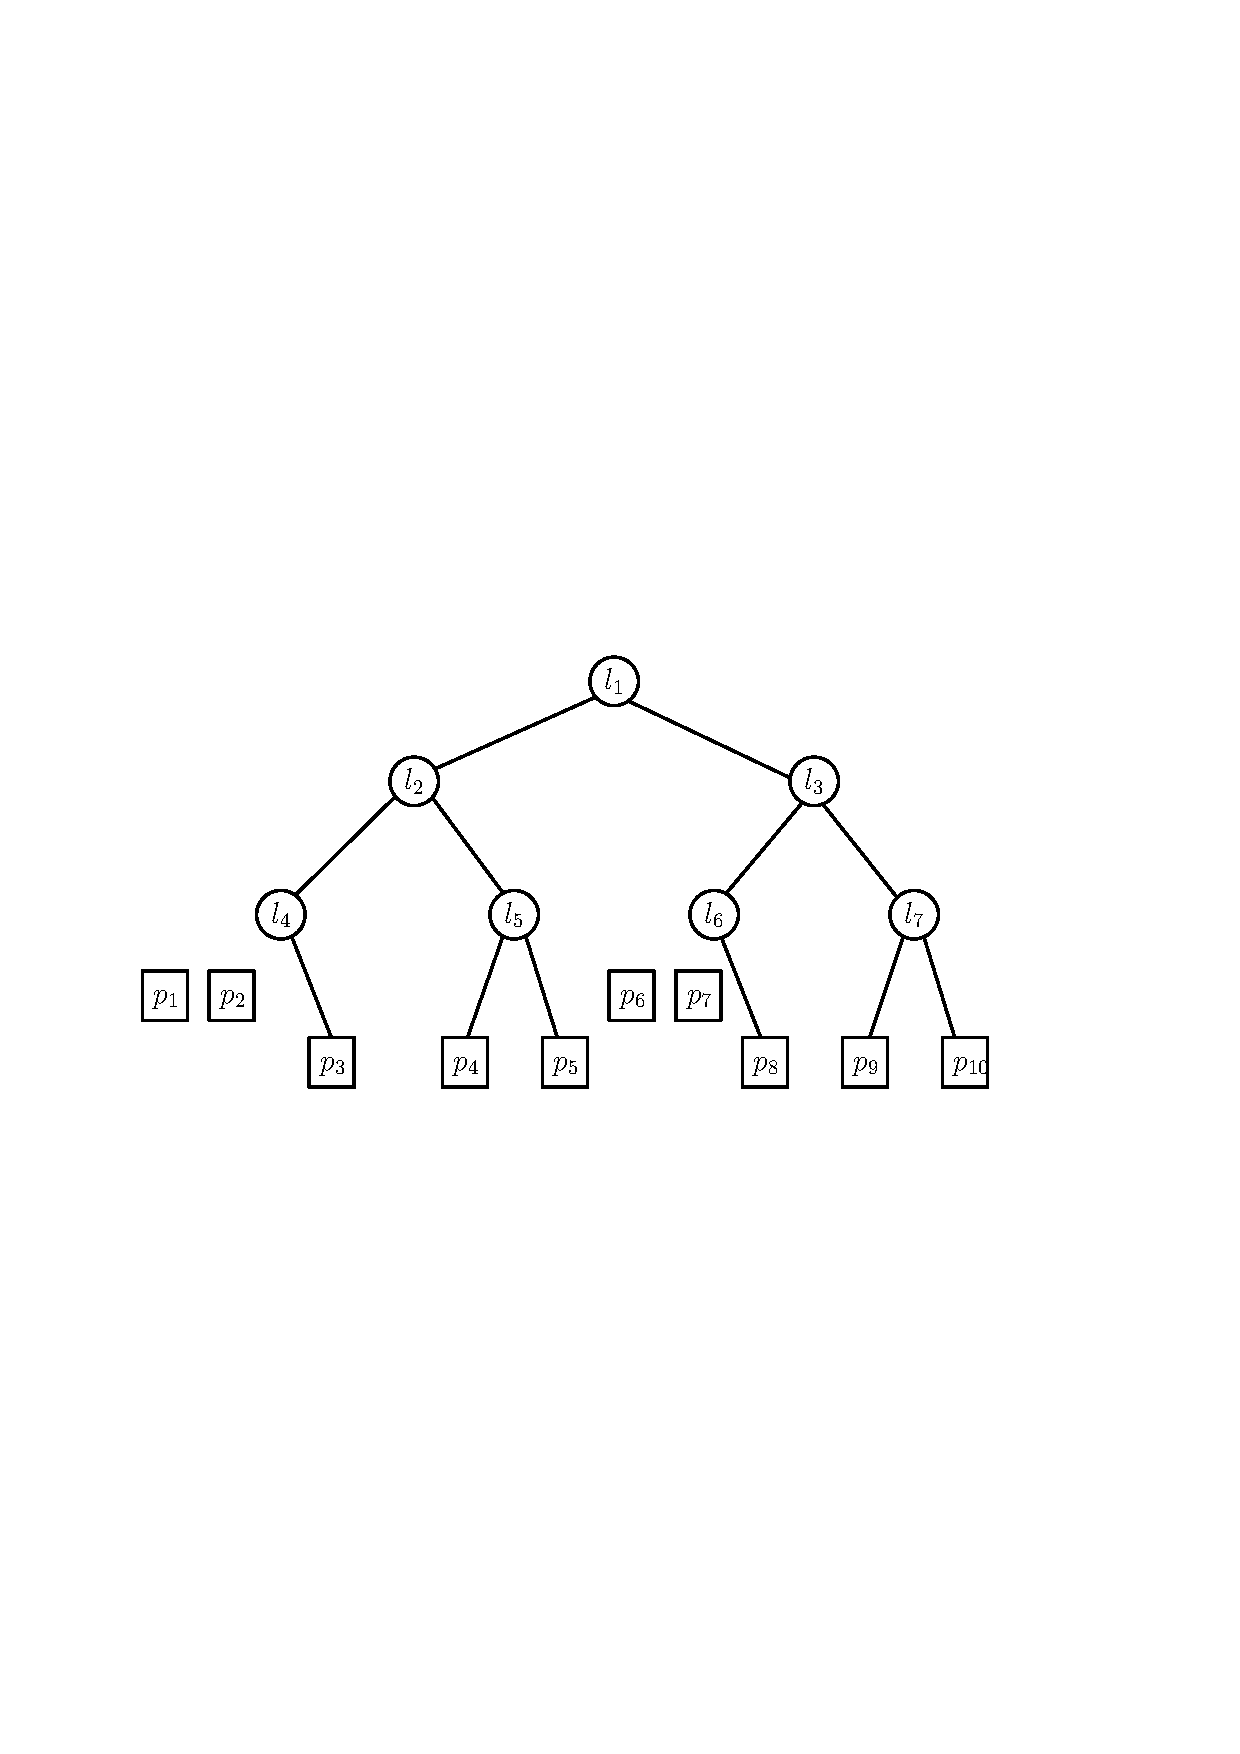
\includegraphics[width=.5\linewidth]{bilder/kdtree7}}
			}
	\end{figure}
	}
	\only<9>{
		\begin{figure}
		\mbox{
			\subfigure{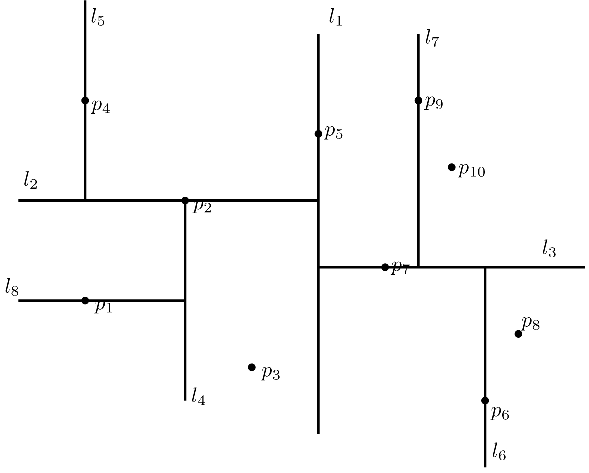
\includegraphics[width=.45\linewidth]{bilder/kd8}}\quad
			\subfigure{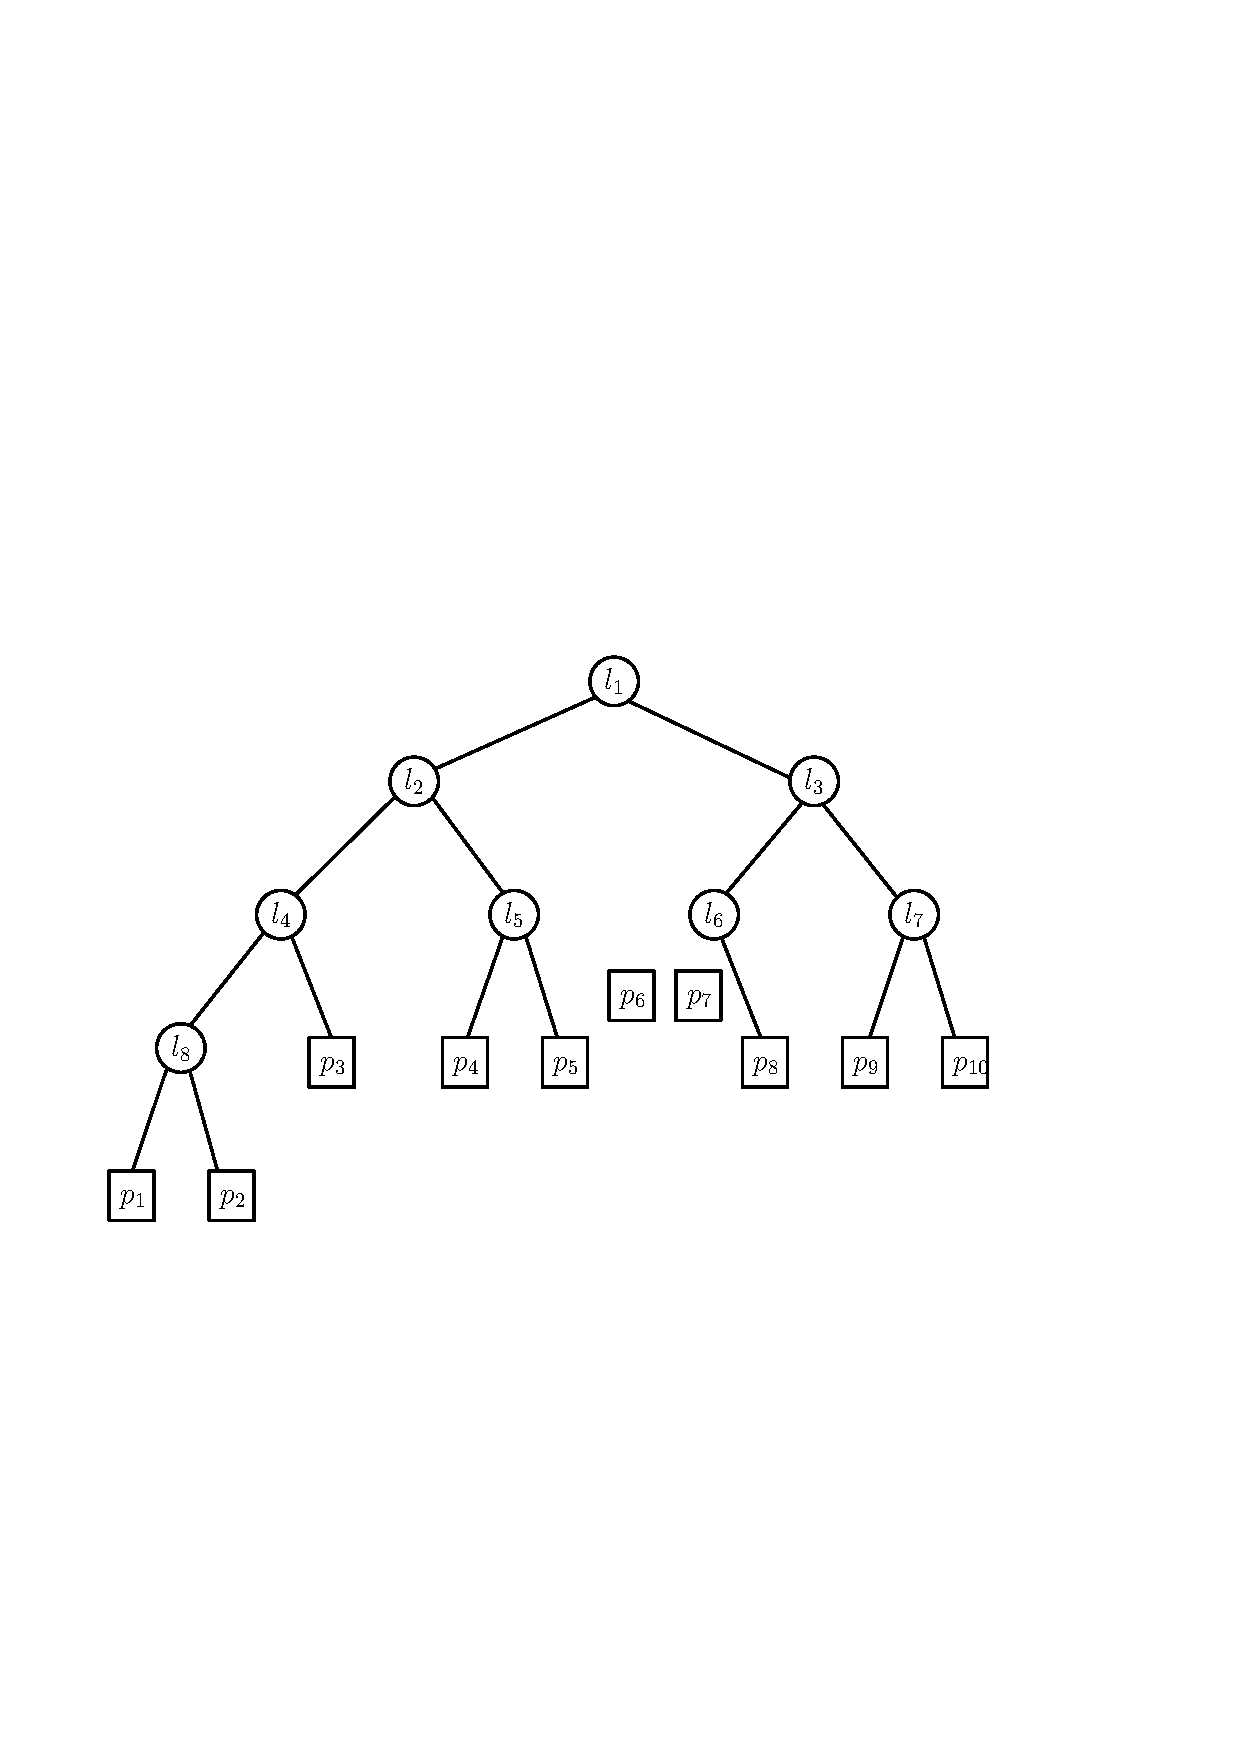
\includegraphics[width=.5\linewidth]{bilder/kdtree8}}
			}
	\end{figure}
	}
	\only<10>{
		\begin{figure}
		\mbox{
			\subfigure{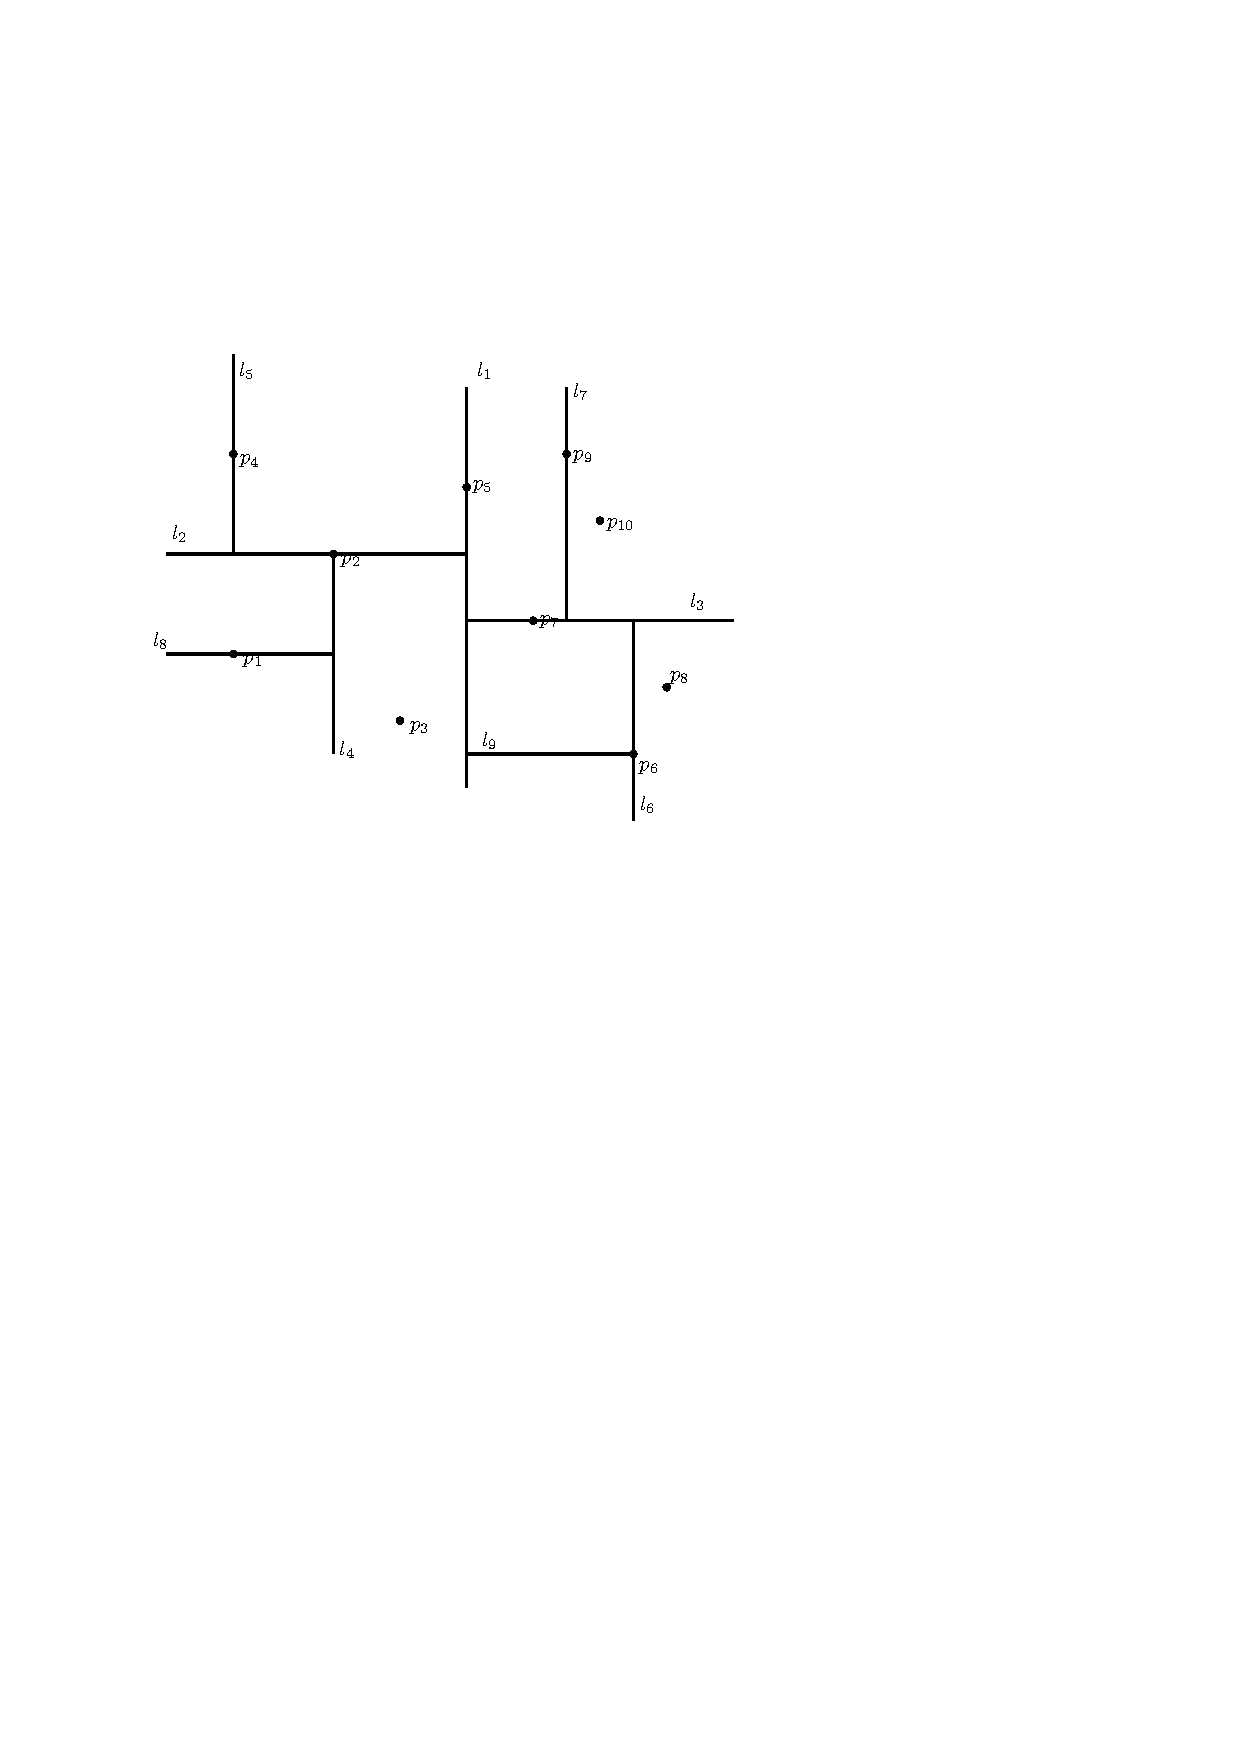
\includegraphics[width=.45\linewidth]{bilder/kd9}}\quad
			\subfigure{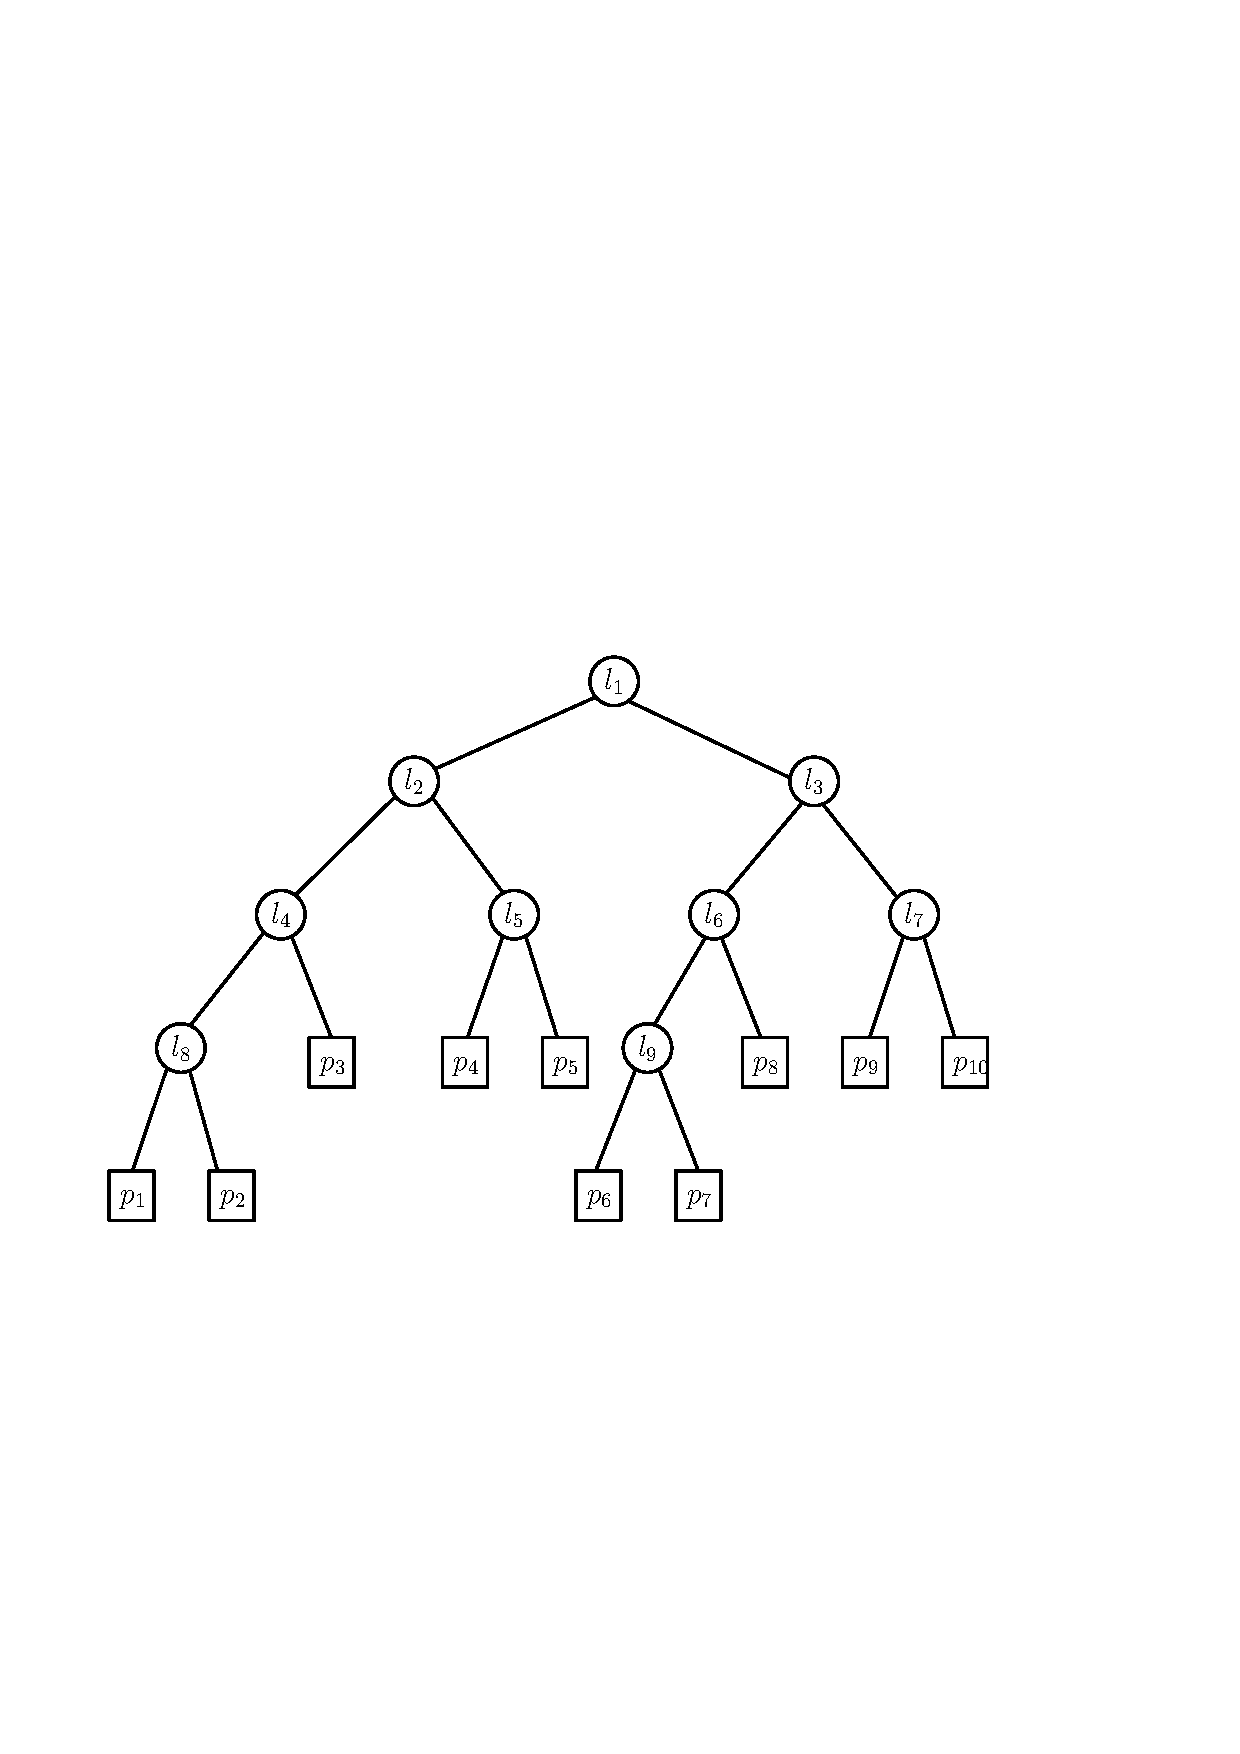
\includegraphics[width=.5\linewidth]{bilder/kdtree9}}
			}
	\end{figure}
	}
	
\end{frame}

\begin{frame}
	\frametitle{kd-Baum - Pseudocode}
	$kdBaumBauen(P, tiefe)$
	\begin{algorithmic}
	\If	{$\mbox{P hat nur einen Punkt}$}
		\State \Return Knoten mit diesem Punkt
	\Else
	\pause
		\If{Tiefe ist gerade}
			\State {Teile P mit einer vertikalen Linie $l$ durch den Median der x-Koordinate in $P_1$ (links von oder auf $l$) und $P_2$ (rechts von $l$)}
		\pause
		\Else
			\State {Teile P mit einer horizontalen Linie $l$ durch den Median der y-Koordinate in $P_1$ (unter oder auf $l$) und $P_2$ (über $l$)}
		\EndIf
		\pause	
		\State $v_{links} \gets kdBaumBauen(P_1, tiefe+1)$
		\State $v_{rechts} \gets kdBaumBauen(P_2, tiefe+1)$
		\pause
		\State {Erstelle Knoten $v$, welches $l$ enthält mit $v_{left}$ als linkem und $v_{right}$ als rechtem Kind von $v$}
		\State \Return $v$
	\EndIf
	\end{algorithmic}
\end{frame}
\begin{frame}
	\frametitle{kd-Baum}
\begin{figure}[htbp]
	\begin{center}
  	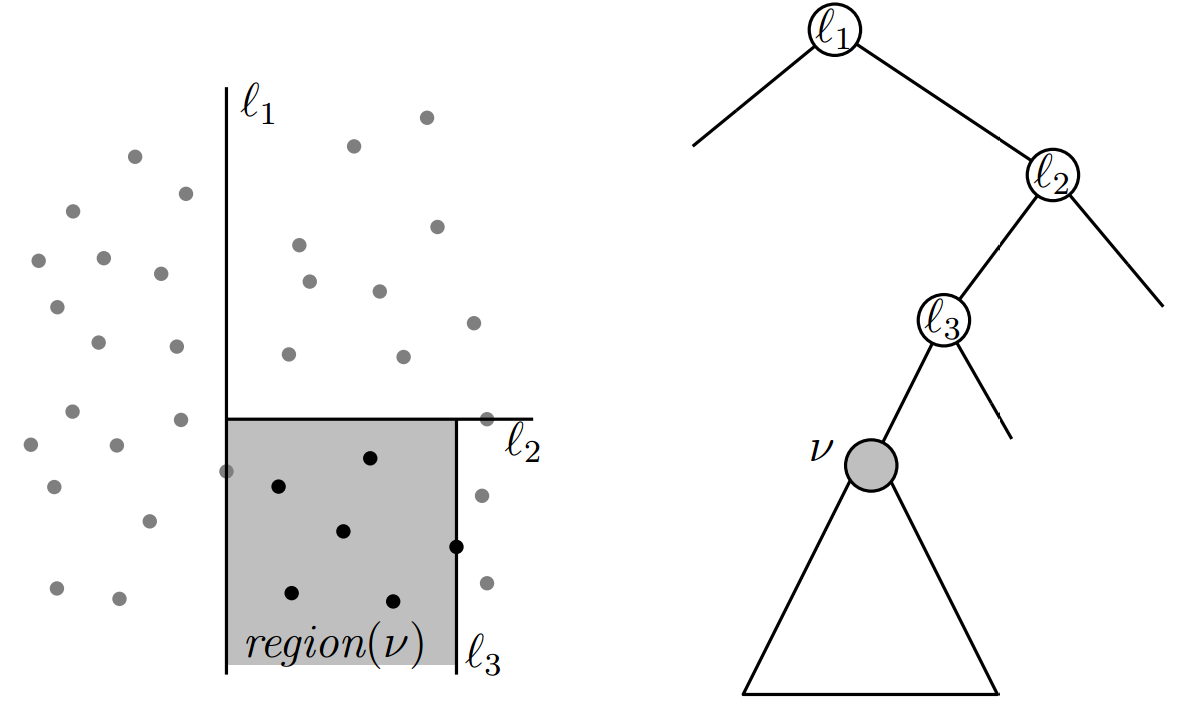
\includegraphics[width=.8\linewidth]{bilder/regionv.png}
	\end{center}
\end{figure}
\end{frame}

\begin{frame}
	\frametitle{kd-Baum}
\begin{figure}[htbp]
	\begin{center}
  	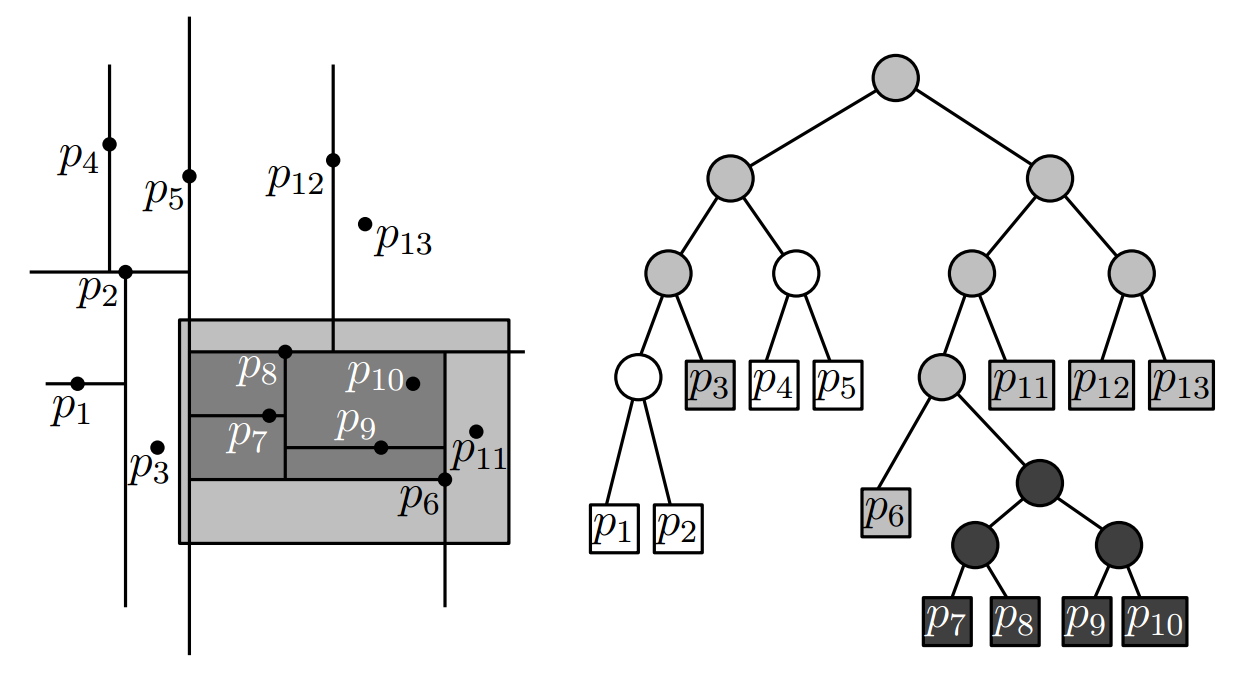
\includegraphics[width=.8\linewidth]{bilder/kdsearch.png}
	\end{center}
\end{figure}
\end{frame}

\begin{frame}
	\frametitle{kd-Baum - Pseudocode}
	Seien v die Wurzel eines (Teil-)Baums und R der Bereich in dem gesucht wird.\\
	$SucheKdBaum(v, R)$
	\begin{algorithmic}
	\If ($v$ ist ein Blatt)
		\State Melde Punkt in $v$, falls es in R liegt.
	\Else
		\pause
		{\If {$region(lc(v))\mbox{ ist vollständig in } R$}
			\State $MeldeTeilbaum(lc(v))$
			\pause
		\Else
			\If{$region(lc(v)) \mbox{ überschneidet sich mit } R$}
				\State $SucheKdBaum(lc(v),R)$				
			\EndIf
		\EndIf}
		\pause
		\State $\mbox{Das ganze dann nochmal äquivalent mit rc(v)}$
	\EndIf
	\end{algorithmic}
\end{frame}

\begin{frame}
	\frametitle{kd-Baum - Laufzeit}
	Kurz noch einige ungezeigte Behauptungen:
	\begin{itemize}
		\item Ein kd-Baum braucht $O(n)$ Speicher
		\item Ein kd-Baum lässt sich in $O(n*log(n))$ erstellen
		\item Eine Bereichssuche in einem kd-Baum liegt in $O(\sqrt{n}+k)$
	\end{itemize}
\end{frame}